\chapter{مکانیک و طراحی صنعتی}

این فصل به تشریح بدنه‌ی ساعت و قسمت‌های مکانیکی آن می‌پردازد. قسمت‌های مکانیکی شامل بدنه‌ی اصلی، دریچه‌ی پشتی و نحوه‌ی سرهم شدن قطعات دیگر است.
\section{بدنه‌ی اصلی}
بدنه‌ی اصلی به قسمتی اطلاق می‌شود که از بیرون دیده می‌شود و بزرگترین قطعه است. طراحی این قطعه از صفر در نرم‌افزار \lr{Solid Works} انجام شده است که مطرح‌ترین نرم‌افزار در زمینه‌ی مکانیک و طراحی صنعتی است. برای ساخت بدنه و بخش‌های مکانیکی نیز از فناوری چاپ سه بعدی بهره بردم.

بدنه‌ی اصلی باید:
\begin{multicols}{2}
\begin{enumerate}
	\item محلی برای نصب صفحه نمایش داشته باشد.
	\item  بتواند \pcbf را درون خود جا دهد و مانع چرخش و جابجایی آن شود.
	\item محلی برای اتصال کابل \lr{USB} داشته باشد.
	\item محلی برای جریان هوا داشته باشد. زیرا مدار شارژ باعث افزایش دما می‌شود.
	\item محلی برای اتصال بند داشته باشد.
	\item زیبایی بصری داشته باشد
	\item بیش از حد بزرگ نباشد.
\end{enumerate}
\end{multicols}

برای حصول موارد فوق، چندین نمونه بدنه‌ی مختلف طراحی و چاپ شد تا در هر نسخه، بهبودی نسبت به نسخه‌ی قبلی حاصل شود تا هر چه بهتر شروط فوق ارضا شوند.

\subsection{نسخه‌های اولیه}

در ابتدا یک نمونه‌ی اولیه برای تست کلی بدنه و جانمایی \pcbf و صفحه نمایش طراحی و ساخته شد. تصویر این نمونه‌ی اولیه را می‌توان در شکل ؟ مشاهده کرد.

\begin{figure}[h]
	\centering
	\begin{subfigure}{0.44\textwidth}
		\centering
		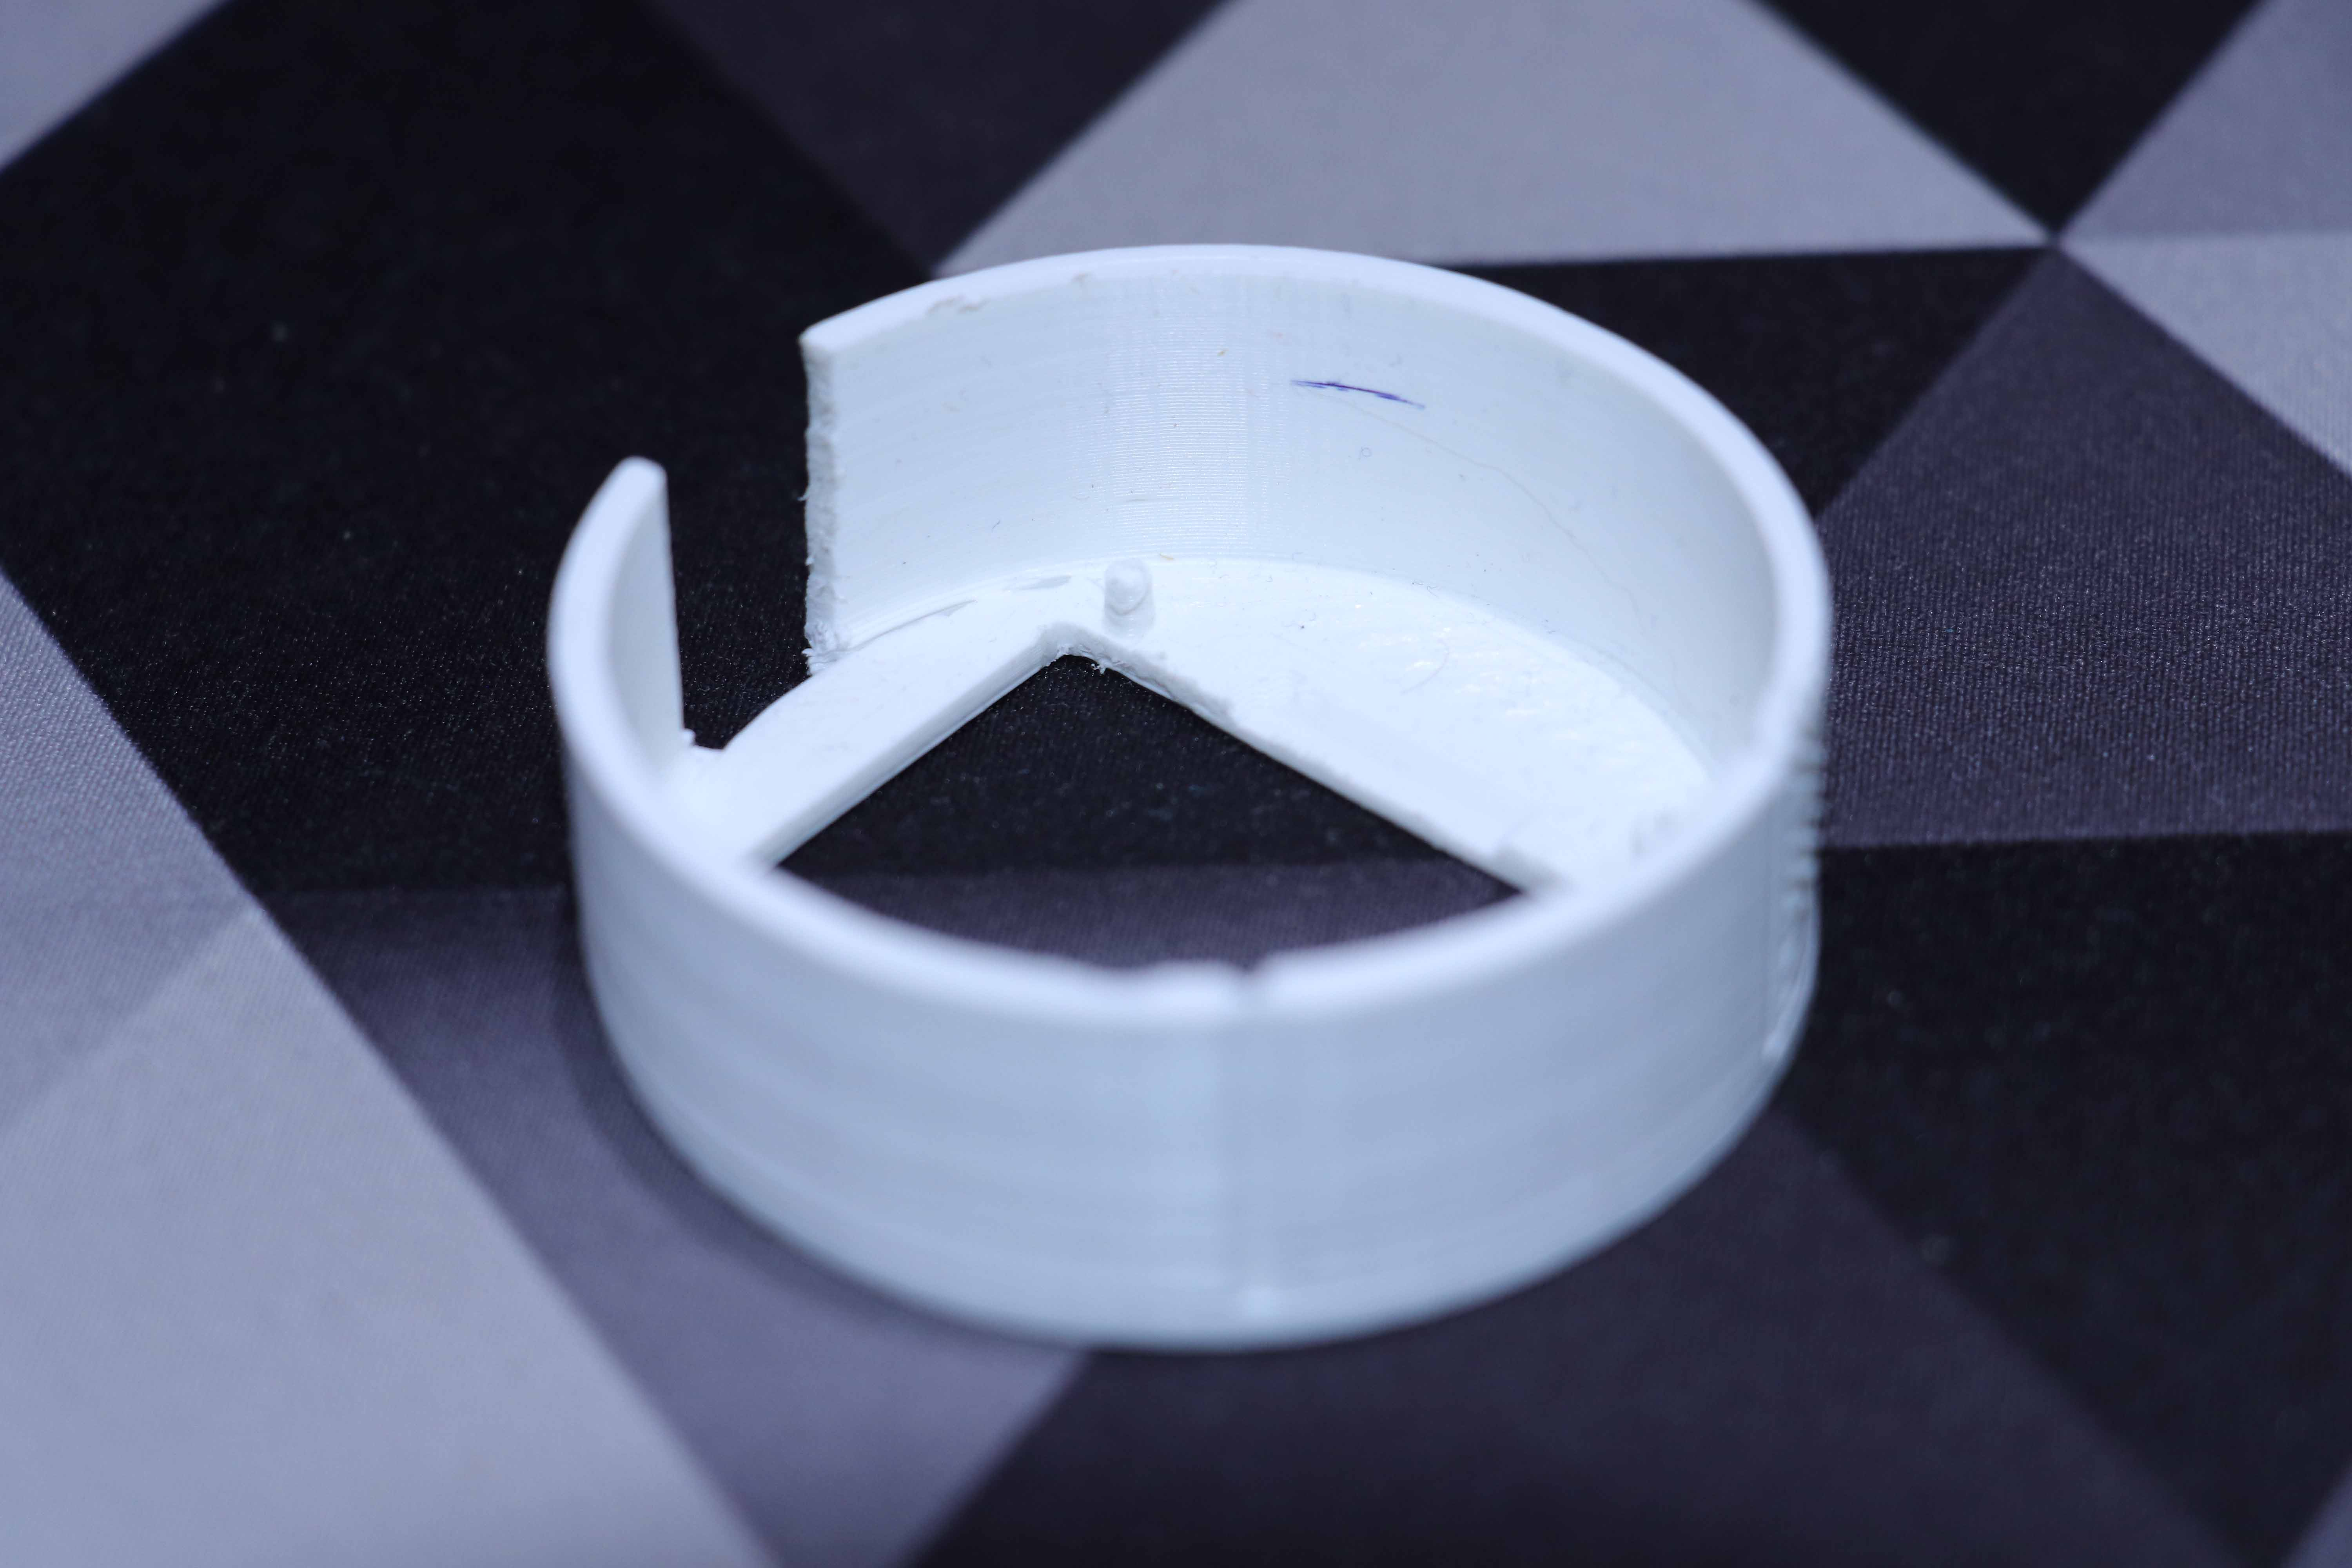
\includegraphics[width=\linewidth]{body_main_v1_back}
		\caption{نمای پشت}
		%\label{fig:oled_image}
	\end{subfigure}
	\begin{subfigure}{0.44\textwidth}
		\centering
		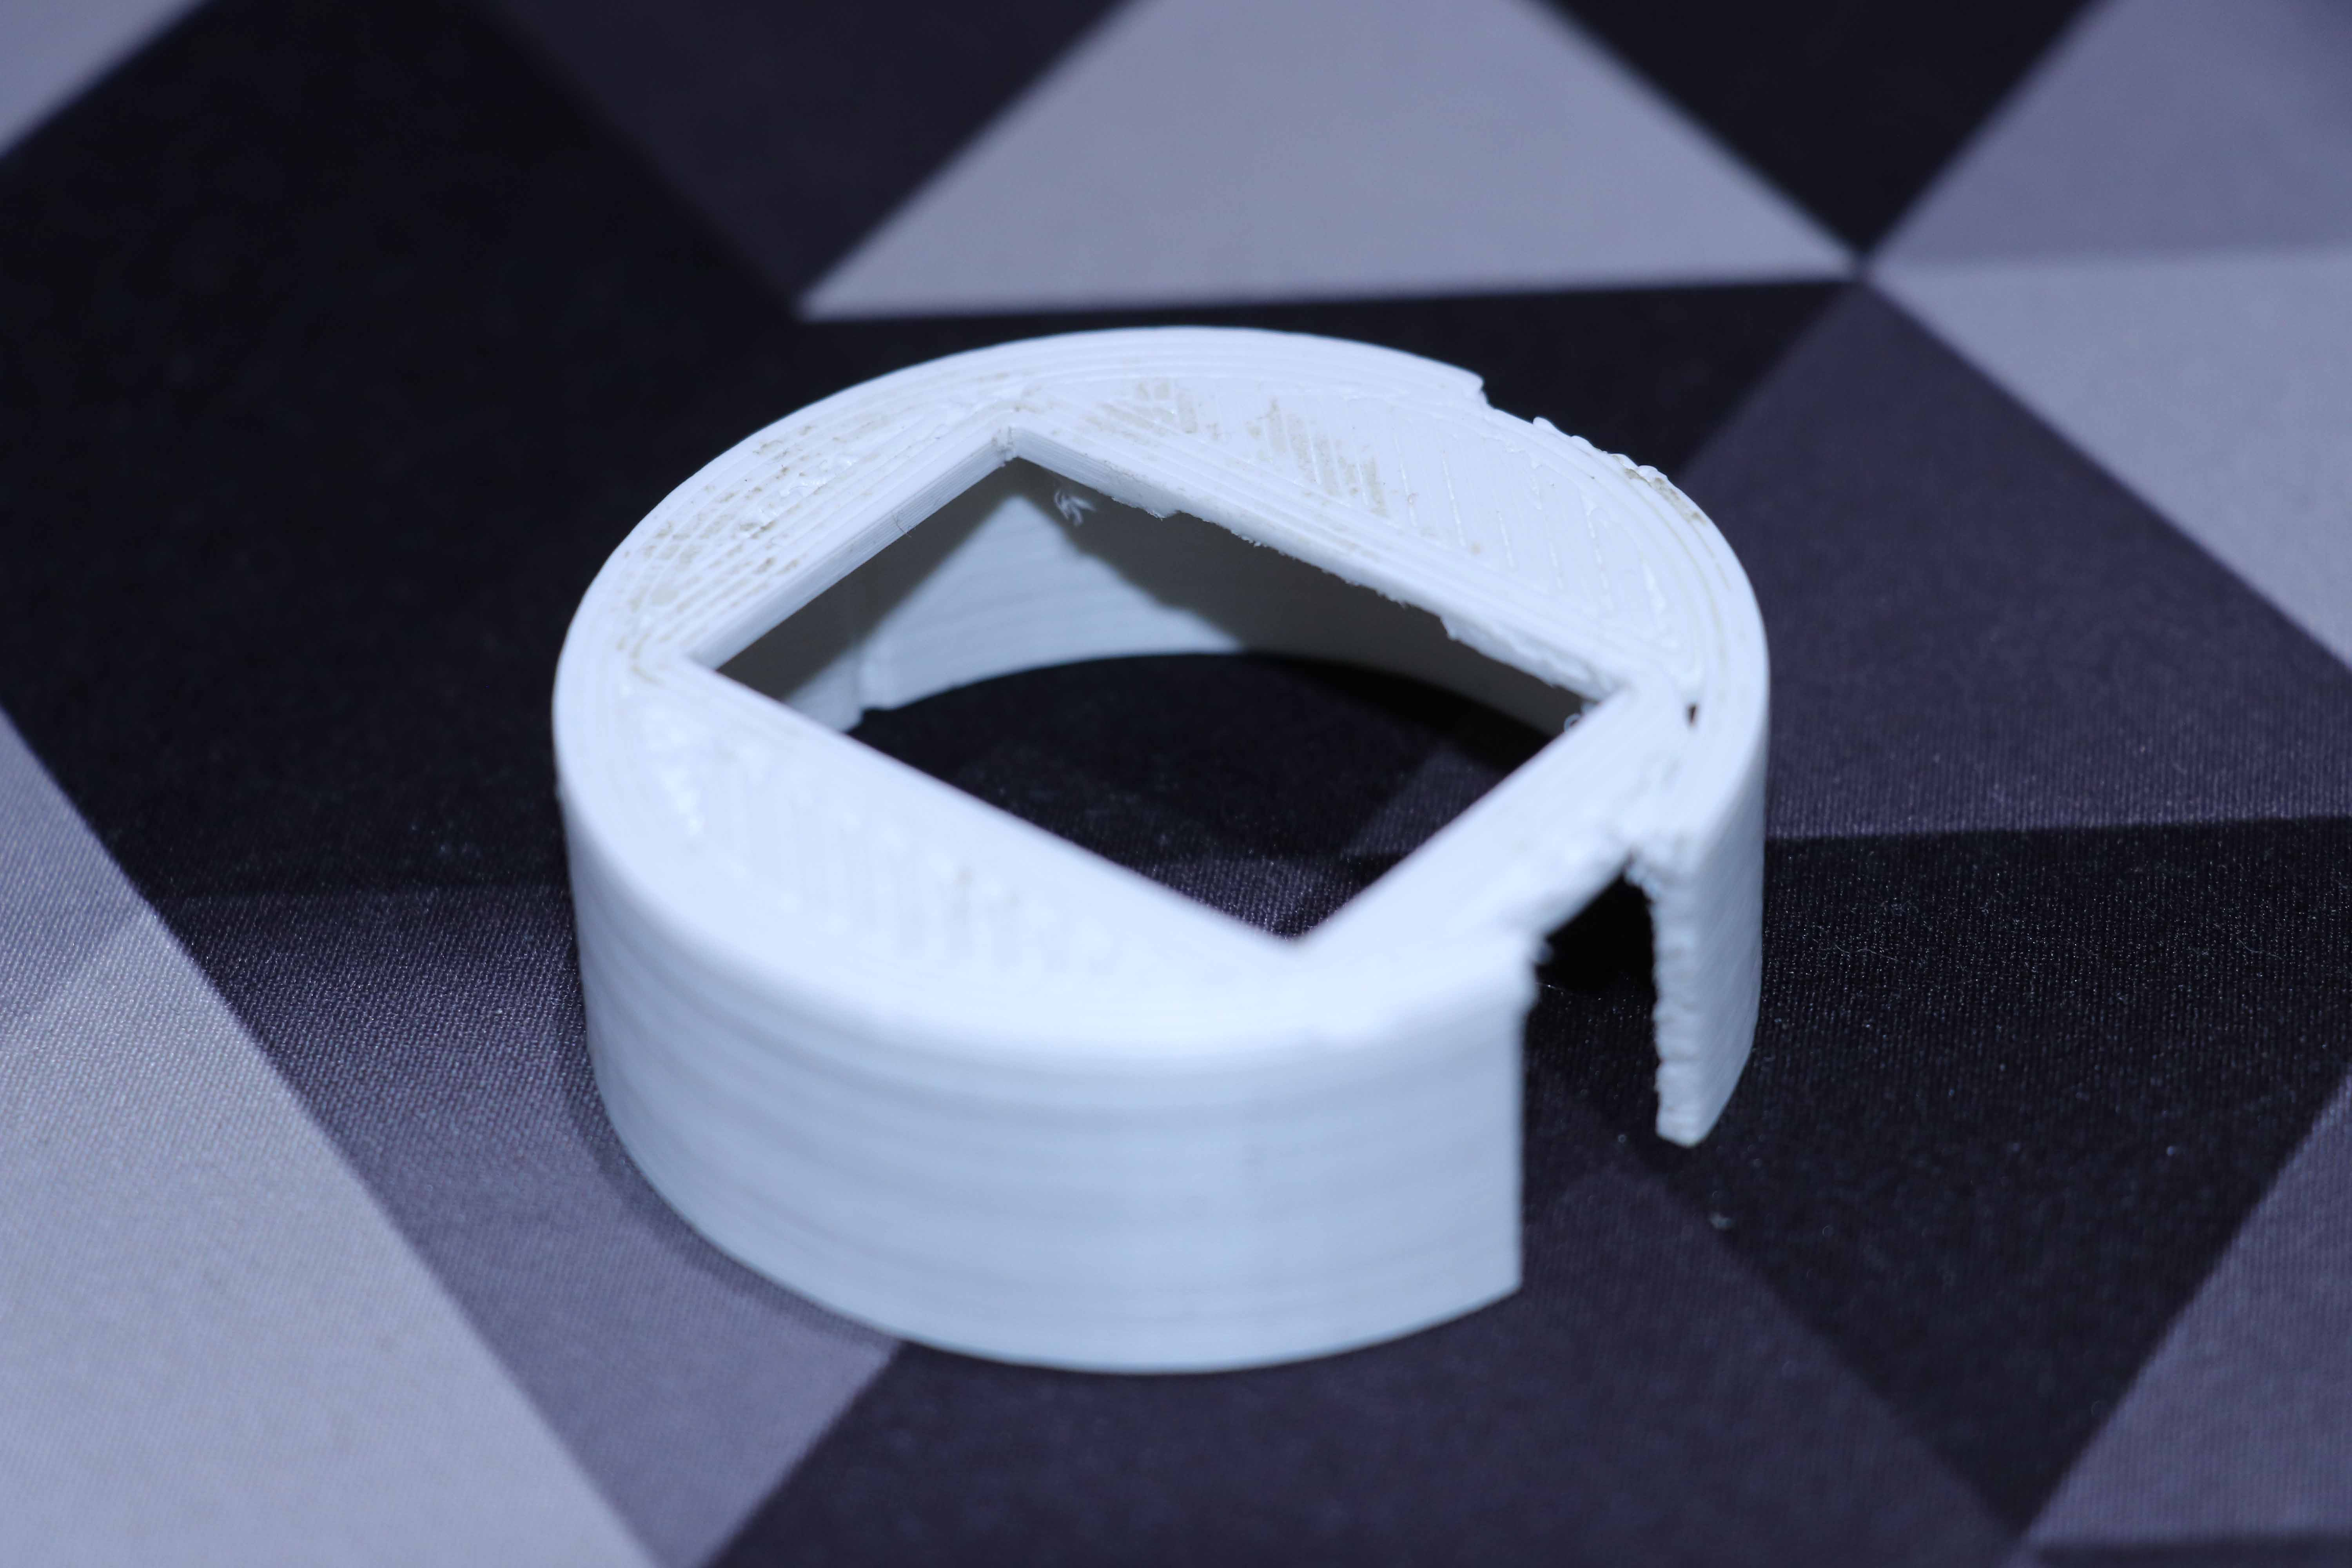
\includegraphics[width=\linewidth]{body_main_v1_front}
		\caption{نمای روبرو}
		%\label{fig:oled_real}
	\end{subfigure}
	\caption{تصاویر بدنه‌ی اصلی نسخه‌ی اول}
	\label{fig:body-v1}
\end{figure}

سپس بعد از نهایی شدن طرح کلی، جزئیات طرح تکمیل شد و نسخه‌ی دوم بدنه به چاپ رسید. تصویر این نسخه در شکل ؟ دیده می‌شود.

\begin{figure}[h]
	\centering
	\begin{subfigure}{0.44\textwidth}
		\centering
		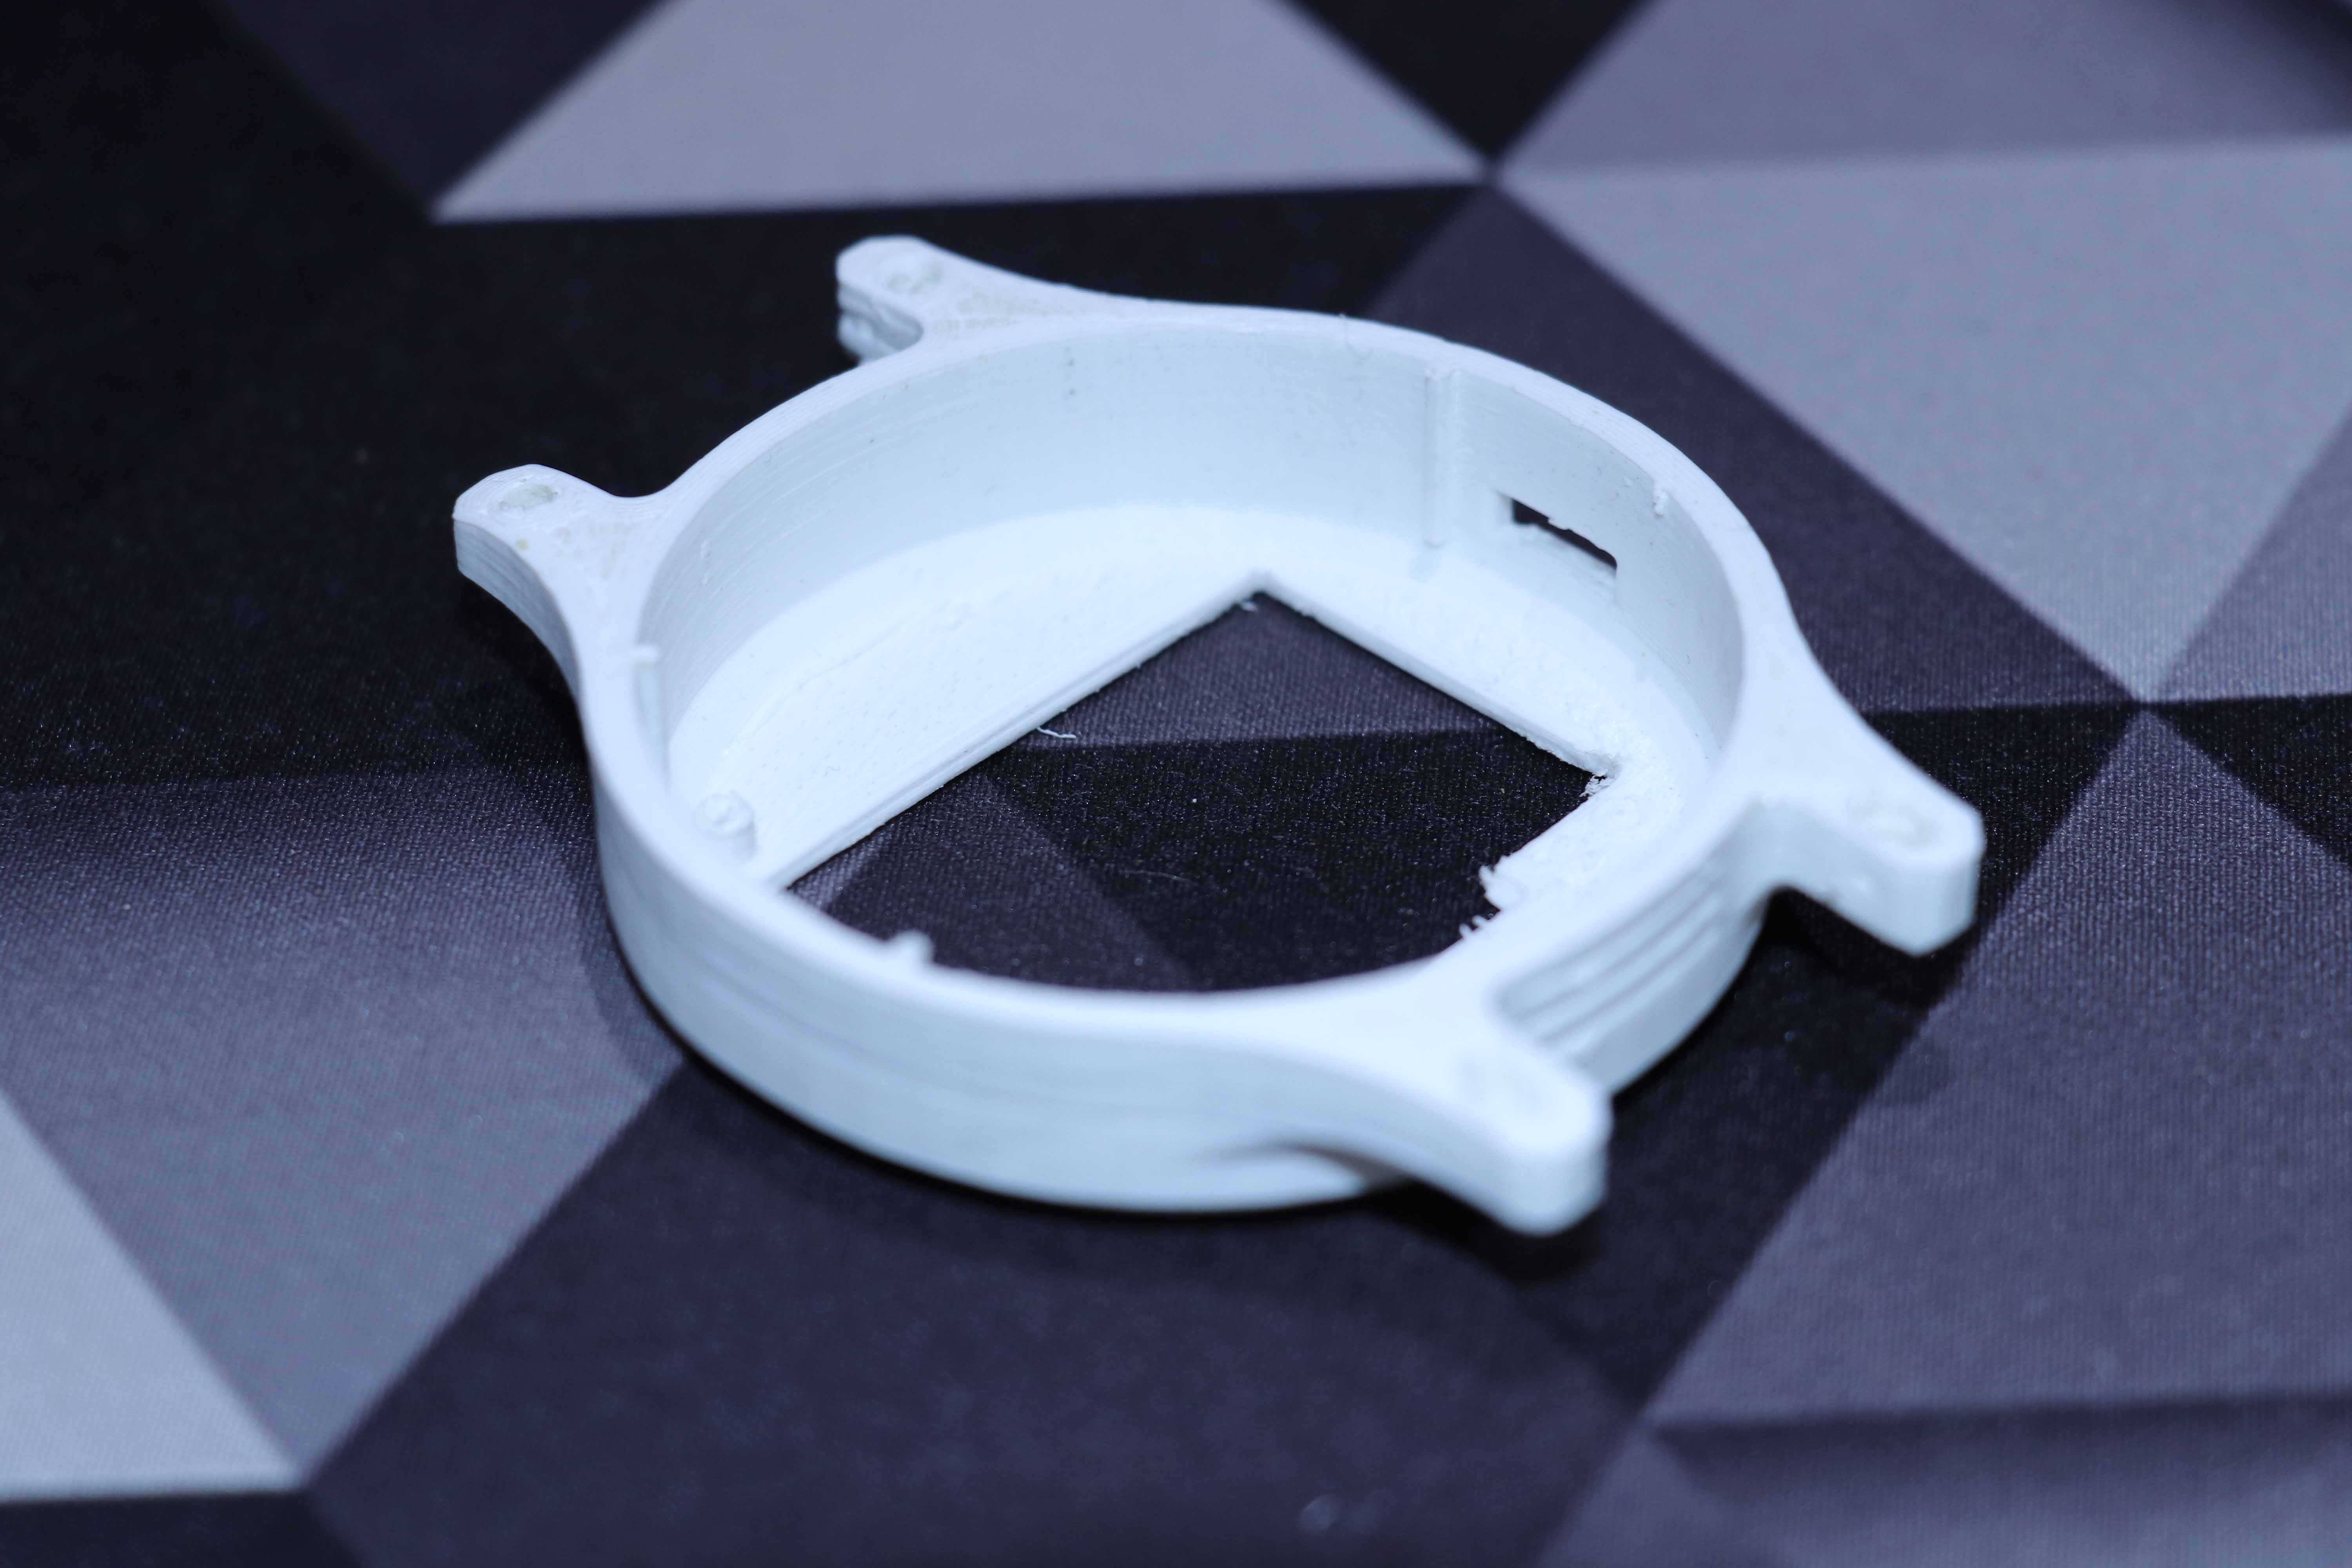
\includegraphics[width=\linewidth]{body_main_v2_back}
		\caption{نمای پشت}
		%\label{fig:oled_image}
	\end{subfigure}
	\begin{subfigure}{0.44\textwidth}
		\centering
		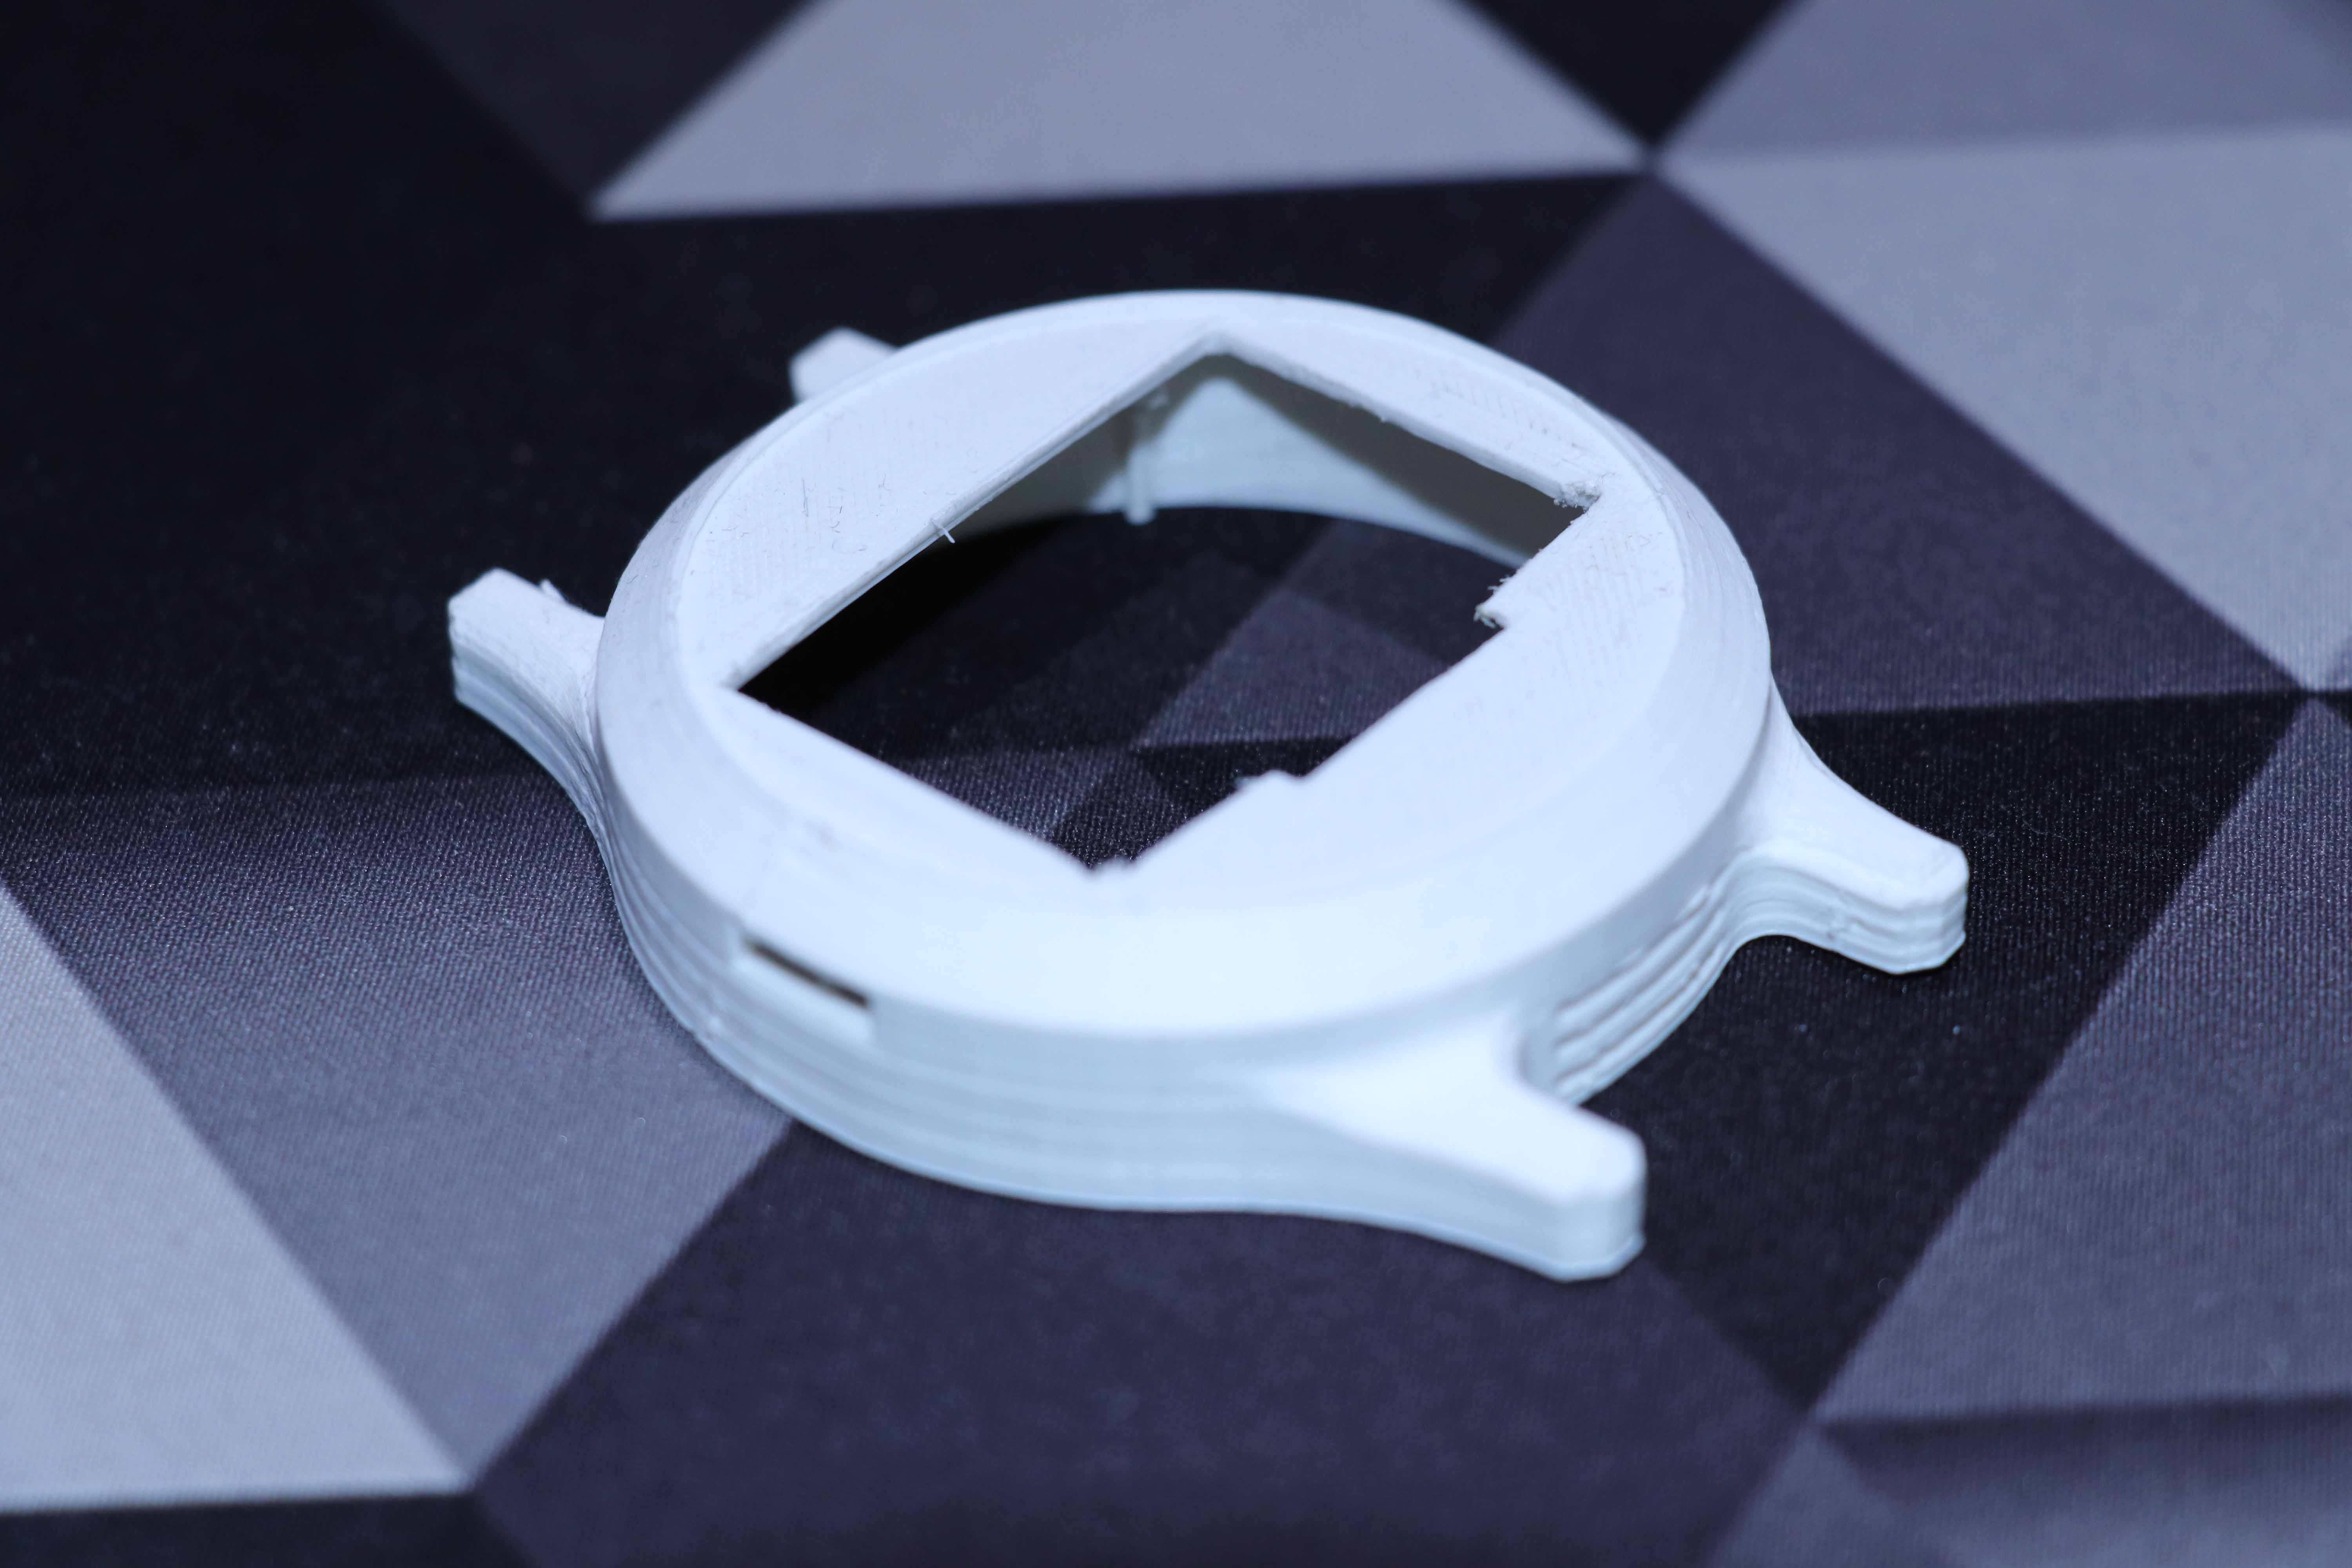
\includegraphics[width=\linewidth]{body_main_v2_front}
		\caption{نمای روبرو}
		%\label{fig:oled_real}
	\end{subfigure}
	\caption{تصاویر بدنه‌ی اصلی نسخه‌ی دوم}
	\label{fig:body-v2}
\end{figure}

این نسخه ایراداتی داشت، از جمله اینکه قسمت مربوط به محل اتصال بند بیش از حد بزرگ بود از زیبایی بصری می‌کاهید. بعد از برطرف نمودن ایرادات این نسخه، نسخه‌ی سوم به چاپ رسید که شکل ؟ آن را نشان می‌دهد.

\begin{figure}[h]
	\centering
	\begin{subfigure}{0.44\textwidth}
		\centering
		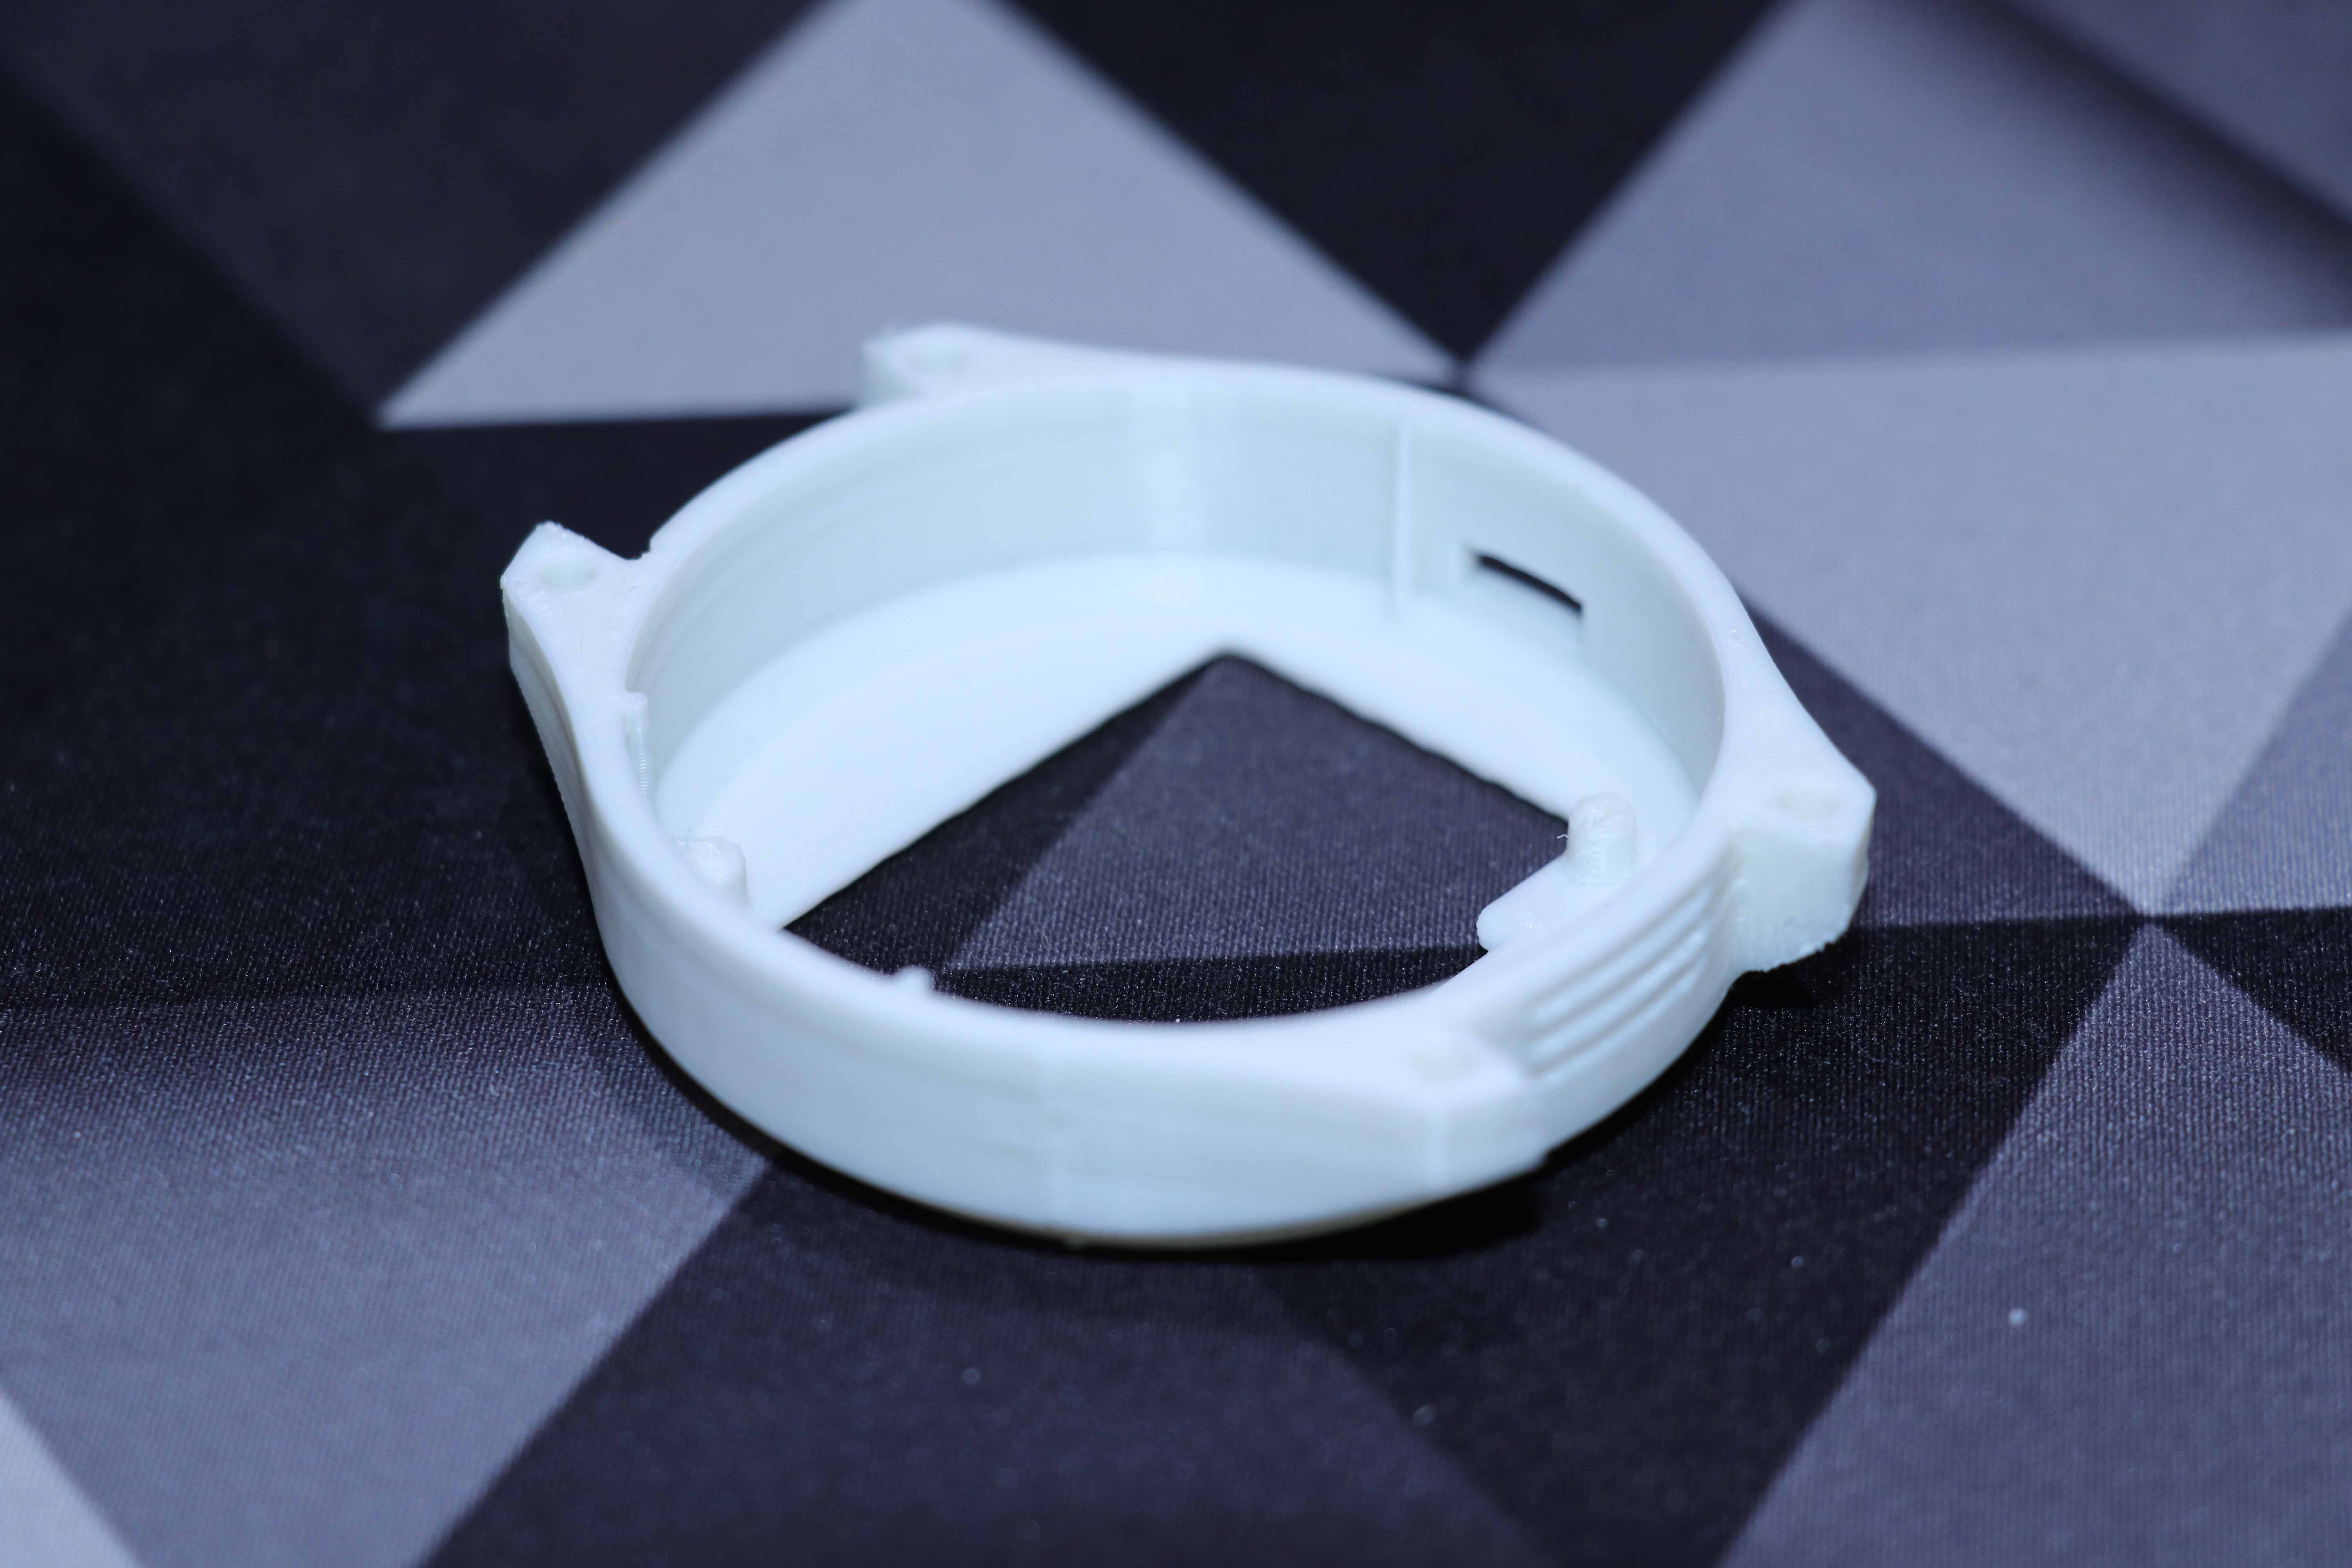
\includegraphics[width=\linewidth]{body_main_v3_back}
		\caption{نمای پشت}
		%\label{fig:oled_image}
	\end{subfigure}
	\begin{subfigure}{0.44\textwidth}
		\centering
		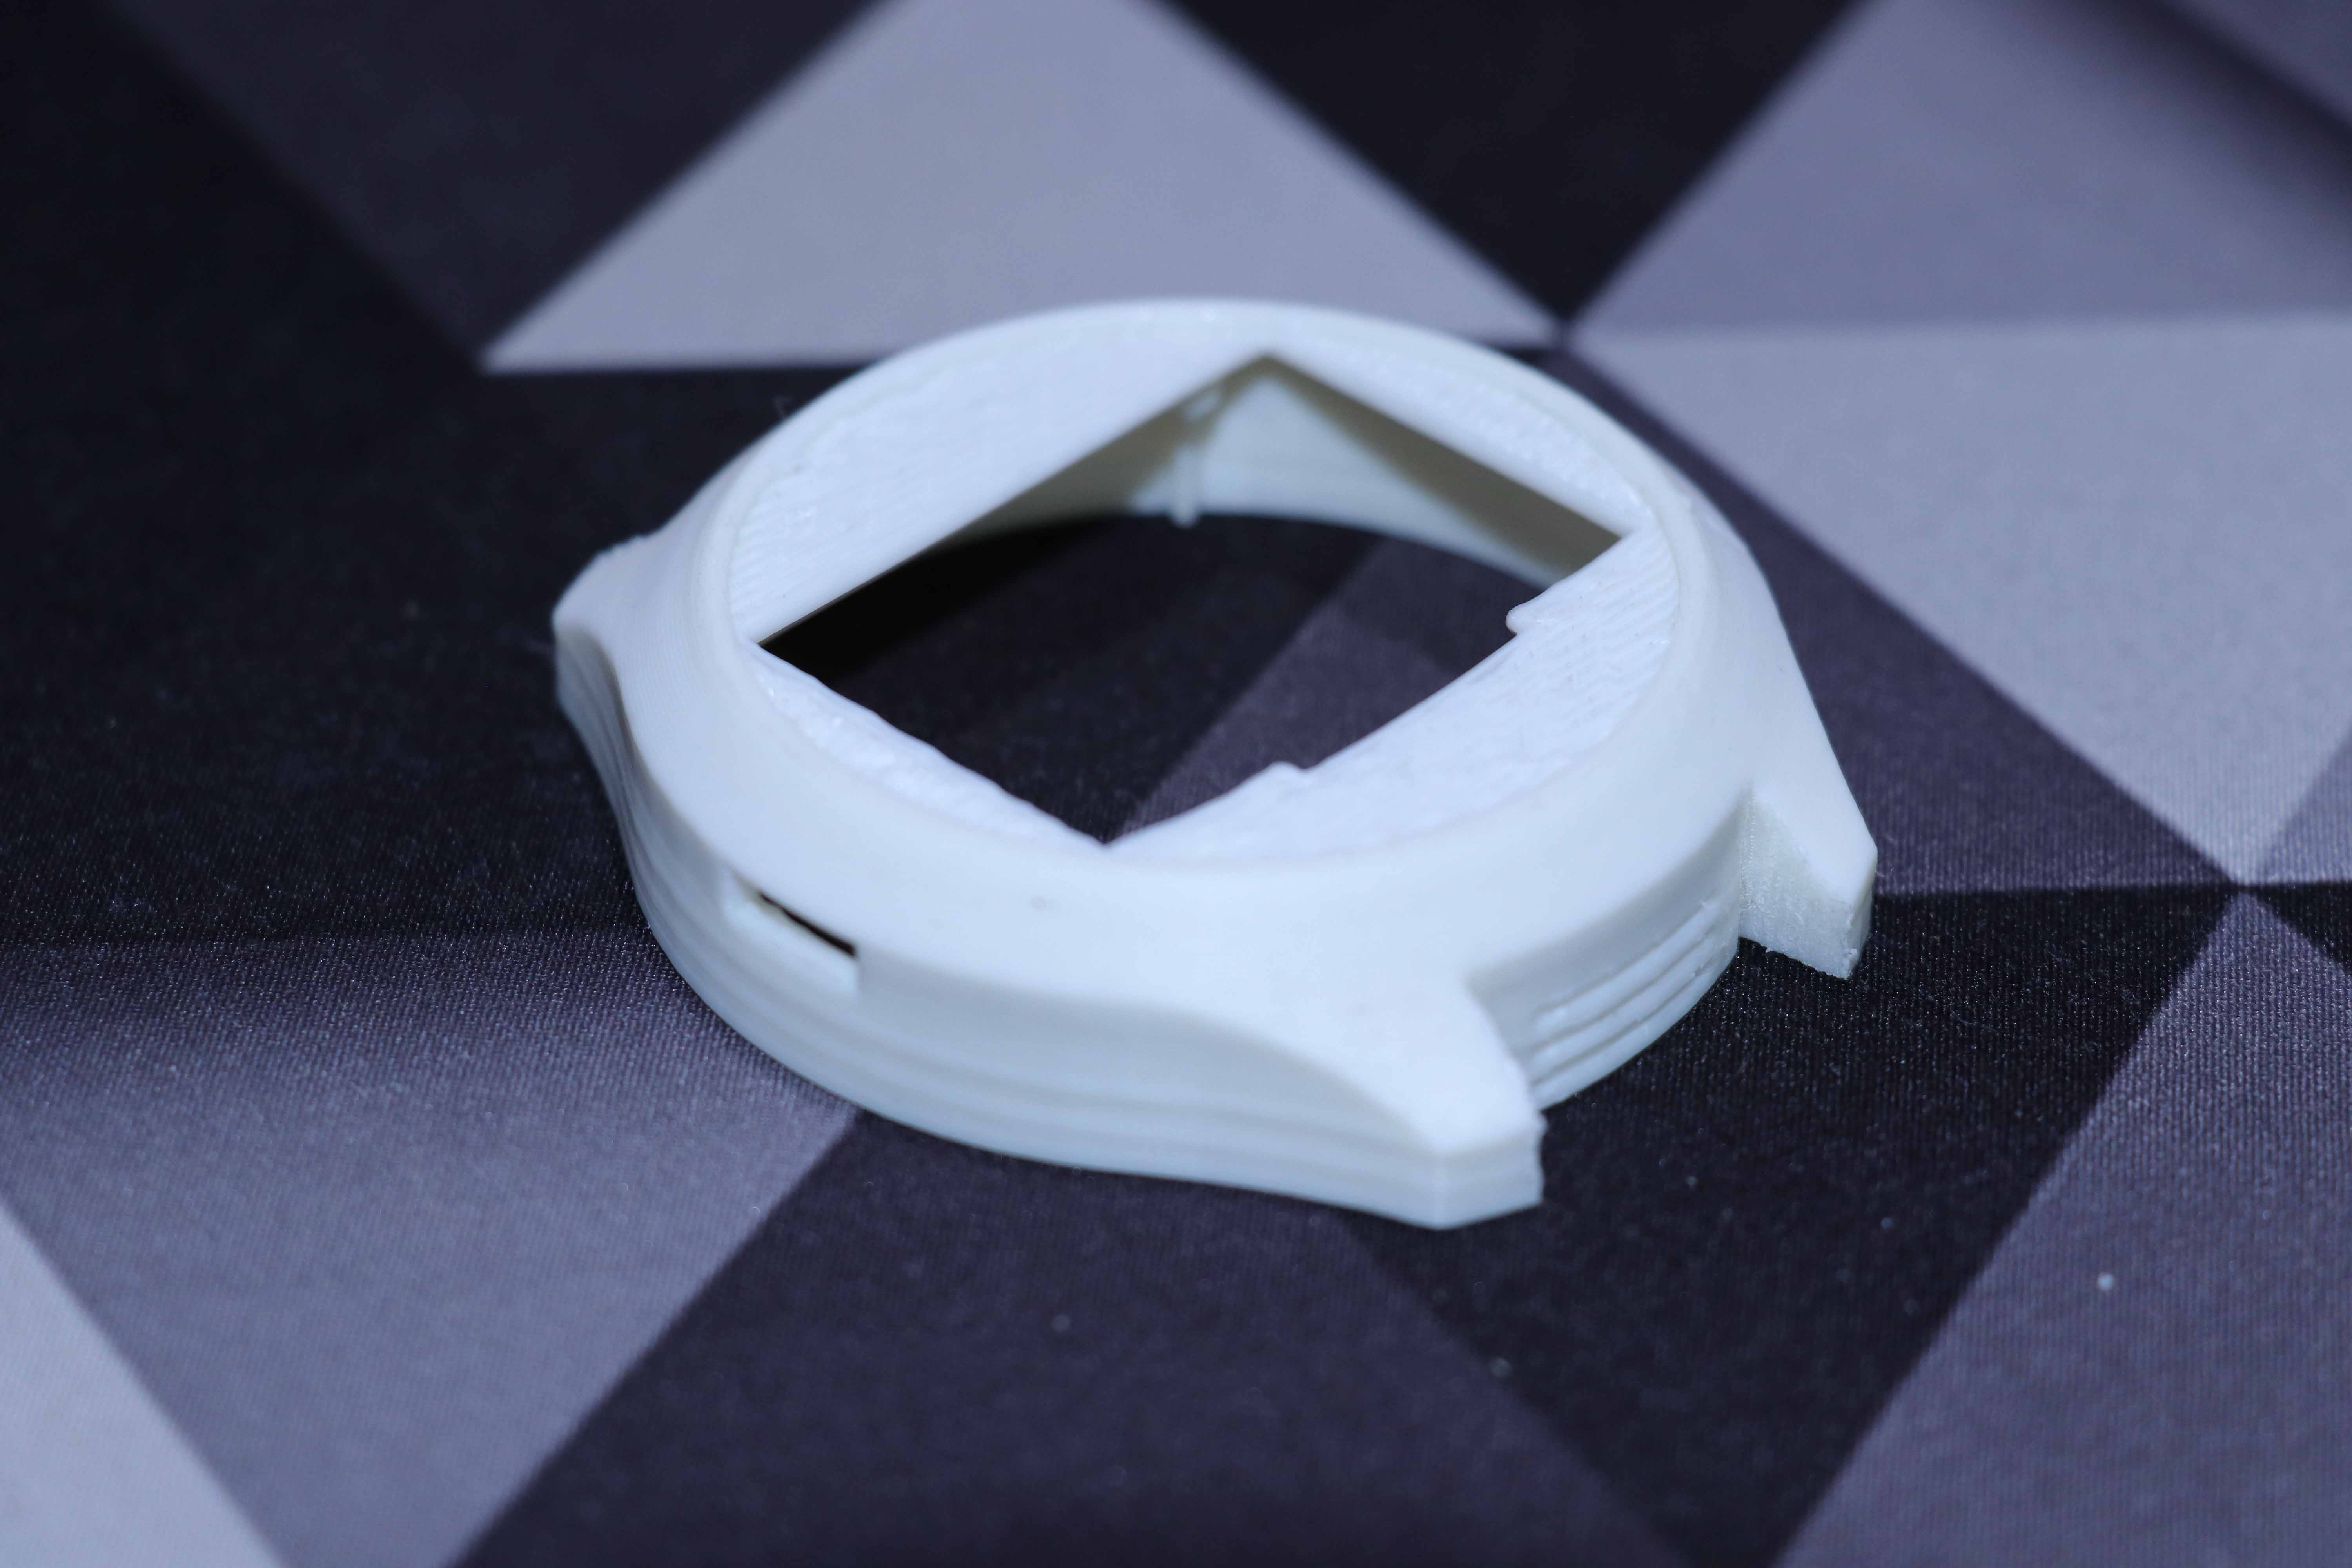
\includegraphics[width=\linewidth]{body_main_v3_front}
		\caption{نمای روبرو}
		%\label{fig:oled_real}
	\end{subfigure}
	\caption{تصاویر بدنه‌ی اصلی نسخه‌ی سوم}
	\label{fig:body-v3}
\end{figure}

این نسخه تقریبا تمام شرایط فوق را ارضا می‌کرد. جانمایی حسگر \lr{PPG} تنها موردی بود که باید انجام میشد. بعد از افزودن این قسمت، نسخه‌ی چهارم و نهایی آماده شد.

\subsection{نسخه نهایی}

شروط بحث شده در بالا را برای نسخه‌ی نهایی بررسی می‌کنیم.
\begin{enumerate}
	\item محل نصب صفحه نمایش: \\
	از سمت بیرون یک مستطیل خالی شده است که تا صفحه نمایش در آن قرار گیرد. از داخل هم سه استوانه منطبق بر سه سوراخ صفحه نمایش وجود دارد تا آن را در جای خود نگه دارد. اگر به تصویر صفحه نمایش (شکل \ref{fig:oled_image}) دقت کنید، پایین آن زائده‌ای برای اتصال سیم‌های فلت به صفحه نمایش قرار دارد. این زائده به شکل یک برش مستطیلی کوچک از صفحه‌ی فوقانی بدنه جدا شده است. شکل \ref{fig:body-oled} این قسمت ها را به خوبی نشان می‌دهد.
	
	\begin{figure}[h]
		\centering
		\begin{subfigure}{0.45\textwidth}
			\centering
			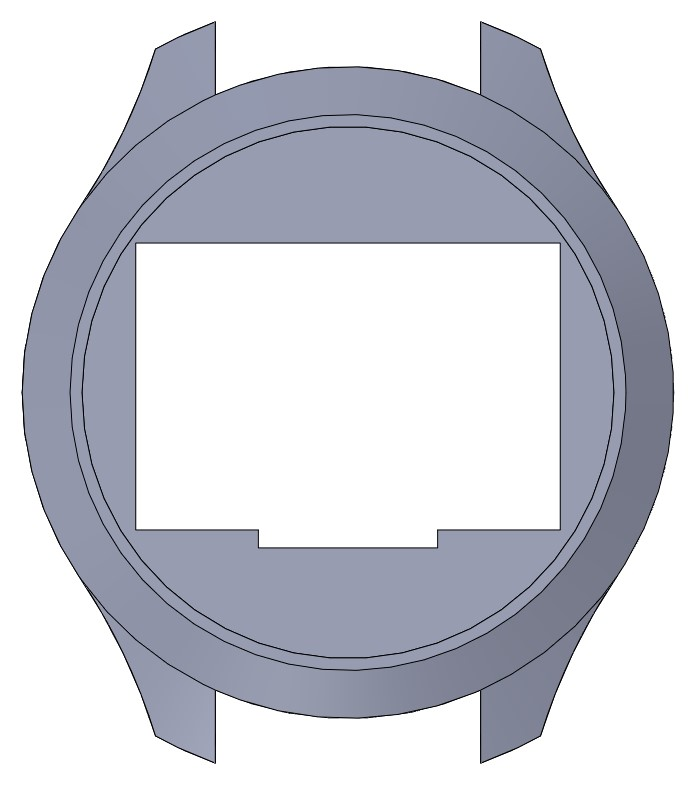
\includegraphics[width=0.78\linewidth]{body_oled}
			\caption{نمای درونی}
			%\label{fig:oled_image}
		\end{subfigure}
		\begin{subfigure}{0.47\textwidth}
			\centering
			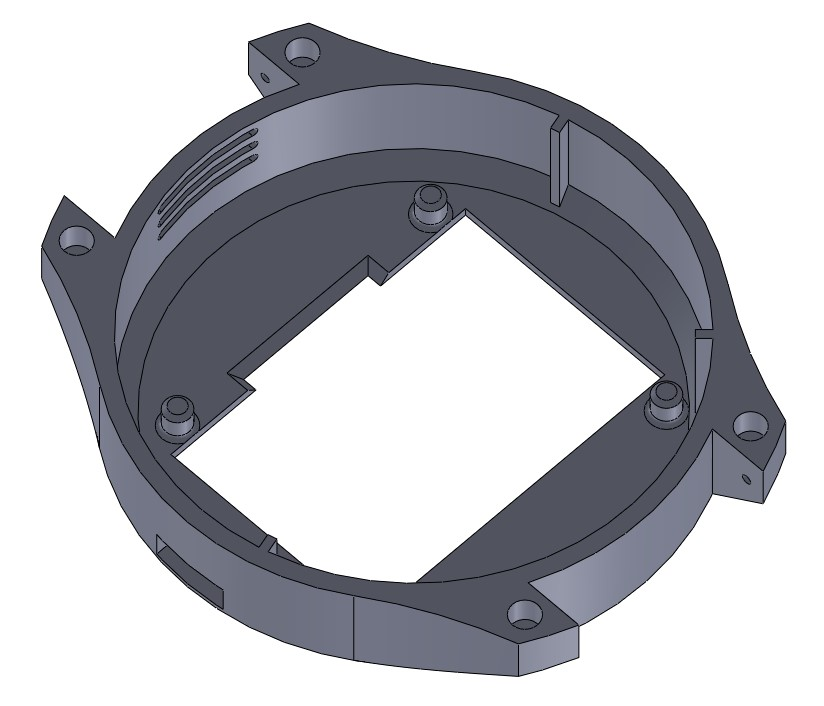
\includegraphics[width=\linewidth]{body_oled2}
			\caption{نمای بیرونی}
			%\label{fig:oled_real}
		\end{subfigure}
		\caption{تصاویر محل نصب صفحه نمایش در بدنه}
		\label{fig:body-oled}
	\end{figure}

	\item  جانمایی \pcbf و جلوگیری از چرخش آن: \\
	بر روی \pcbf سه شیار کوچک وجود دارد. متناظر با آن روی بدنه نیز سه زائده با همان ابعاد تعبیه شده است. این سه زائده مانع چرخش \pcbf در جای خود می‌شوند. تصویر این نگه‌دارنده‌ها در شکل \ref{fig:body-pcb} قابل مشاهده است.
	
	\begin{figure}[h]
		\centering
		\begin{subfigure}{0.44\textwidth}
			\centering
			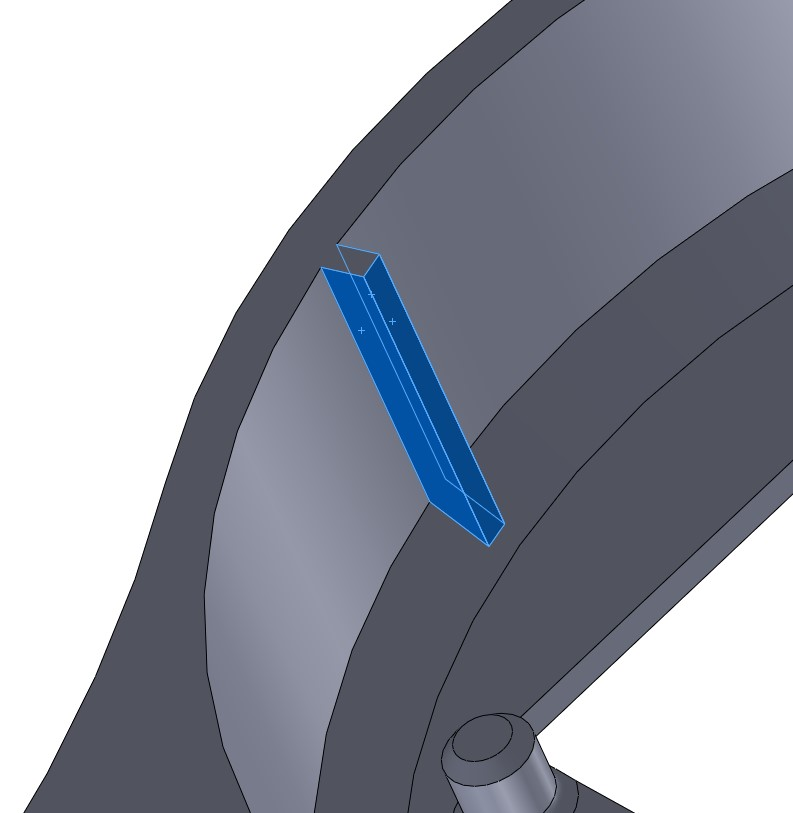
\includegraphics[width=\linewidth]{body_pcb2}
			\caption{نمای درونی}
			%\label{fig:oled_image}
		\end{subfigure}
		\begin{subfigure}{0.44\textwidth}
			\centering
			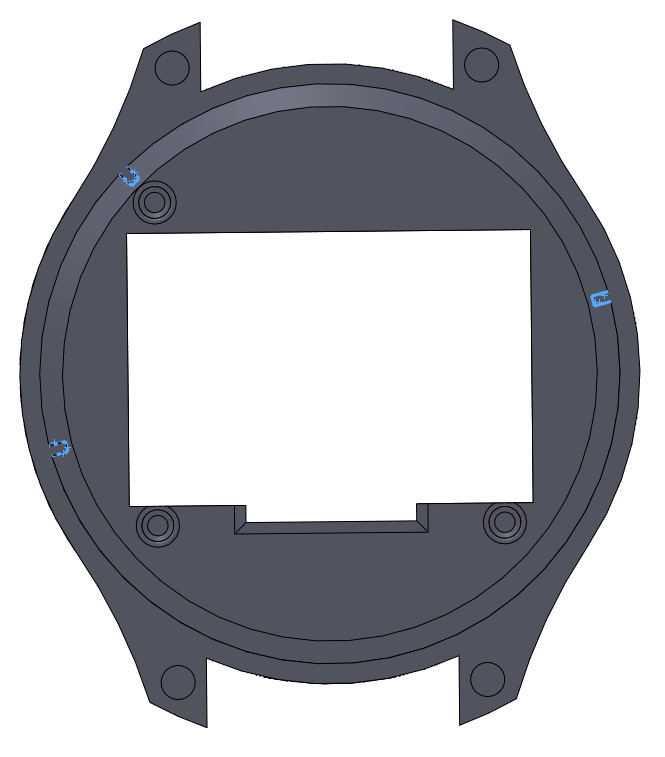
\includegraphics[width=\linewidth]{body_pcb}
			\caption{نمای بیرونی}
			\label{fig:body-pcb-out}
		\end{subfigure}
		\caption{تصاویر محل نصب \pcbf در بدنه}
		\label{fig:body-pcb}
	\end{figure}
	
	\item محل اتصال کابل \lr{USB}: \\
	بر سطح جانبی بدنه یک سوراخ مستطیل شکل به ابعاد کانکتور \lr{micro USB} تعبیه شده است. شکل \ref{fig:body-usb} محل آن روی بدنه را نمایش می‌دهد.

	\begin{figure}[h]
		\centering
		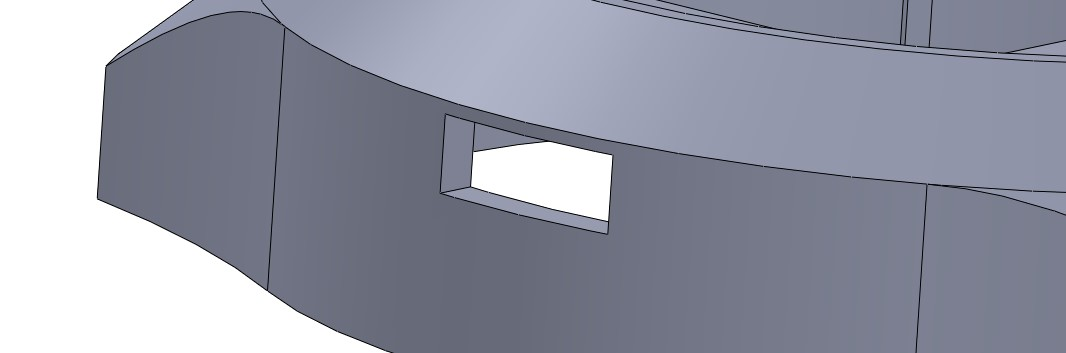
\includegraphics[width=0.75\linewidth]{body_usb}
		\caption{تصویر محل اتصال \lr{USB} در بدنه}
		\label{fig:body-usb}
	\end{figure}
	
	\item محل عبور هوا: \\
	در نزدیکی قطعات مدار شارژ سه شیار برای عبور هوا وجود دارد تا قطعات داخلی به علت بالا رفتن دما آسیب نبینند. این شیارها در شکل \ref{fig:body-air} قابل مشاهده‌اند.
	
	\begin{figure}[h]
		\centering
		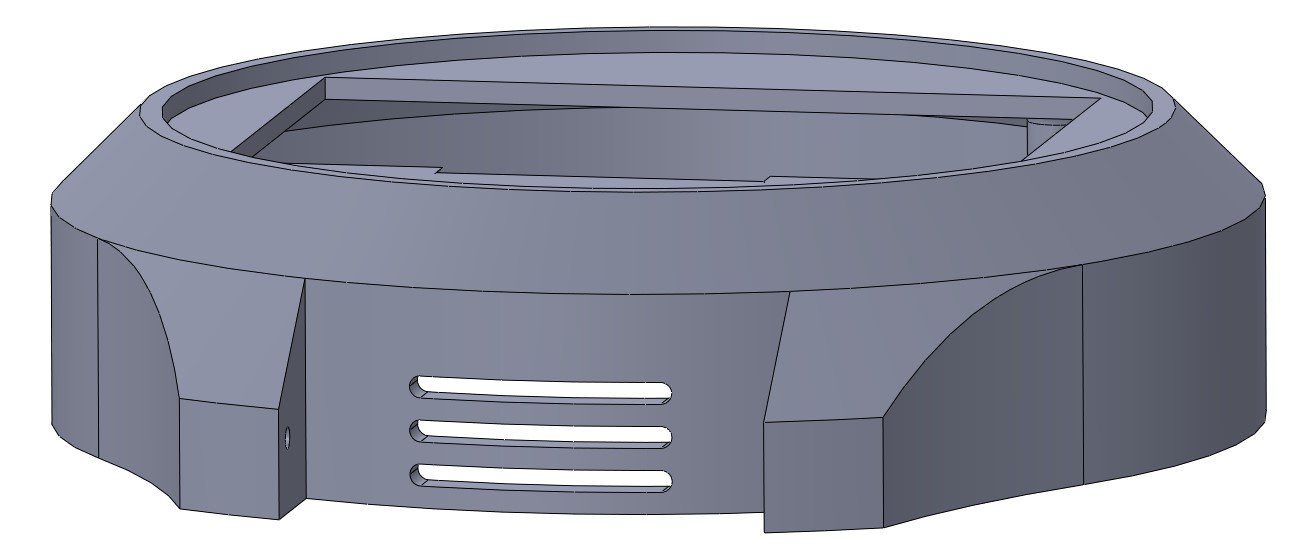
\includegraphics[width=0.75\linewidth]{body_air}
		\caption{تصویر شیارهای عبور هوا}
		\label{fig:body-air}
	\end{figure}

	\item محل اتصال بند: \\
	بندهای موردنظر برای این ساعت مربوط به ساعت هوشمند \lr{Haylou} است. این بندها از جنس پلاستیک هستند. برای اتصال بند به بدنه‌ی اصلی چهار بازوی کوچک به بدنه اضافه شده است. داخل آن‌ها سوراخ‌هایی کوچکی موجود است که پین بند در آن‌ها قرار گیرد. تصویر این بازوها و محل نصب پین را شکل \ref{fig:body-band} مشاهده می‌کنید.
	
	\begin{figure}[h]
		\centering
		\begin{subfigure}{0.4\textwidth}
			\centering
			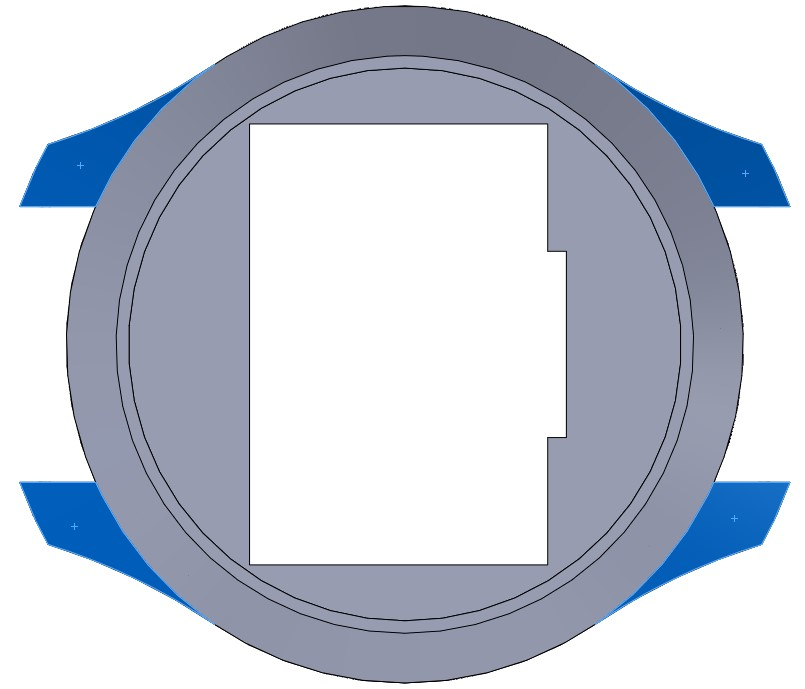
\includegraphics[width=\linewidth]{body_band}
			\caption{چهار بازو برای اتصال بند}
			%\label{fig:oled_image}
		\end{subfigure}
		\begin{subfigure}{0.3\textwidth}
			\centering
			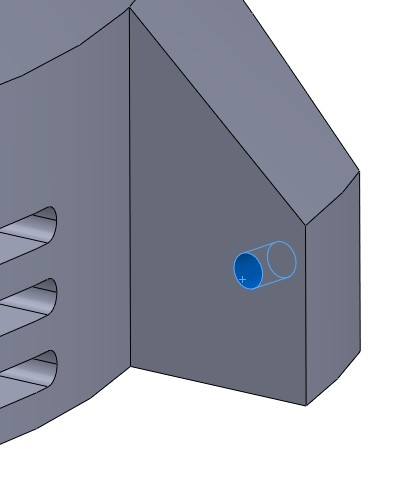
\includegraphics[width=\linewidth]{body_band2}
			\caption{سوراخ های نصب پین}
			%\label{fig:oled_real}
		\end{subfigure}
		\caption{تصاویر محل نصب بند}
		\label{fig:body-band}
	\end{figure}

	\item زیبایی بصری: جای تردید نیست که این طرح زیبا است :)
	\item ابعاد دقیق طرح در بخش‌های بعدی تشریخ خواهد شد؛ اما در مورد تناسب ابعاد، قطر دایره‌ی این ساعت حدود 5 سانتی‌متر است که در مقایسه با ساعت‌های موجود در بازار، مقدار بزرگی نیست و معقول است.
\end{enumerate}

در نهایت تصویر بدنه‌ی اصلی در شکل \ref{fig:body-real} دیده می‌شود. چاپ این نسخه توسط شرکت \lr{PCBWay}\cite{PCBWay} به رایگان انجام شده است. جنس بدنه از رزین است که باعث می‌شود شفاف باشد و داخل آن دیده شود.

	\begin{figure}[h]
		\centering
		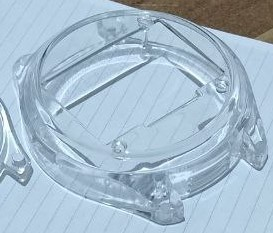
\includegraphics[width=0.5\linewidth]{body_real2}
		\caption{تصویر چاپ شده‌ی نسخه‌ی نهایی بدنه از جنس رزین و شفاف}
		\label{fig:body-real}
	\end{figure}

\section{دریچه‌ی پشتی}
دریچه‌ی پشتی وظیفه دارد تا بر پشت بدنه‌ی اصلی نصب شود و قطعات و تجهیزات داخل ساعت را محافظت کند. از طرفی محل نصب حسگر \lr{PPG} نیز هست. این دو وظیفه را شرح می‌دهیم.

\begin{enumerate}
	\item اتصال به بدنه‌ی اصلی:
	برای اتصال به بدنه‌ی اصلی، چهار استوانه‌ی کوچک بر روی دریچه طراحی شده ‌است. این استوانه‌ها منطبق بر سوراخ‌های روی بدنه است. این سوراخ‌ها در شکل \ref{fig:body-pcb-out} به خوبی دیده می‌شوند. بدین شکل دریچه به بدنه متصل می‌شود. تصویر دریچه در شکل \ref{fig:body-back2main} نشان داده شده‌است.
	
	\begin{figure}[h]
		\centering
		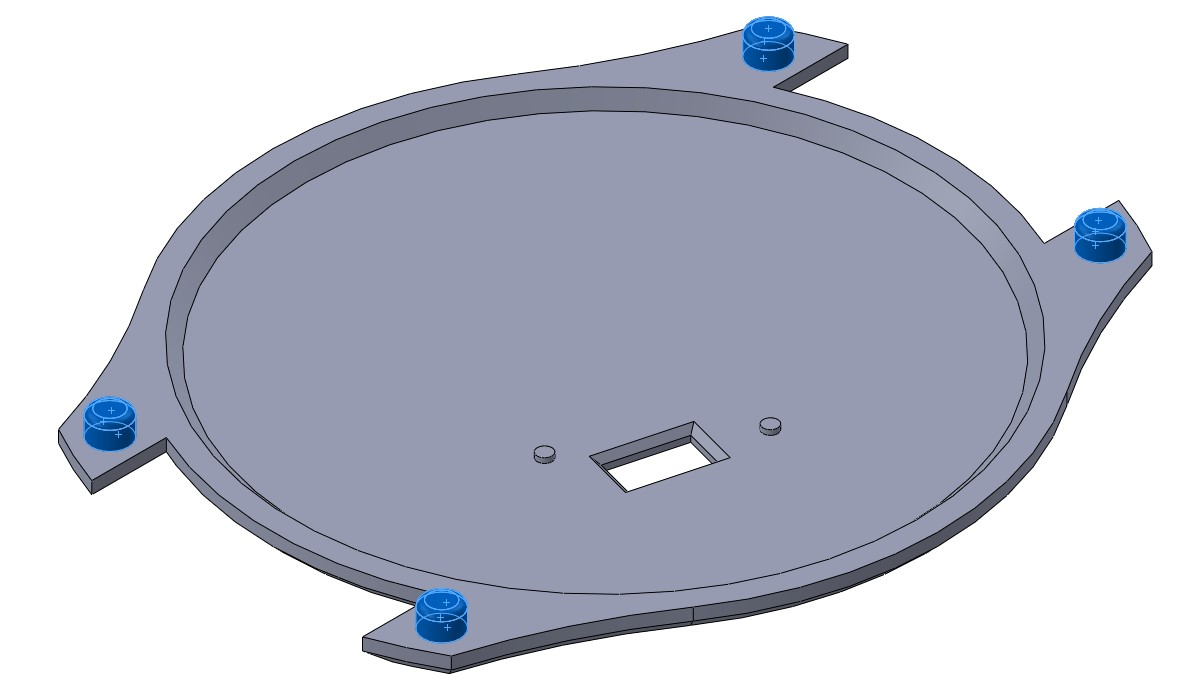
\includegraphics[width=0.7\linewidth]{body_back2main}
		\caption{تصویر استوانه‌های اتصال دریچه به بدنه}
		\label{fig:body-back2main}
	\end{figure}
	
	\item اتصال حسگر \lr{PPG}:
	حسگر باید جایی نصب شود که با پوست تماس مستقیم داشته باشد. لذا بر روی دریچه سوراخ مستطیل شکلی ایجاد شده است تا محل نصب حسگر باشد. دو زائده‌ی کوچک نیز در نزدیکی آن قرار دارد تا منطبق بر سوراخ‌های روی حسگر باشد. این سوراخ‌ها در شکل \ref{fig:ppg_image} قابل مشاهده ‌اند. شکل \ref{fig:body-ppg} محل نصب حسگر را نشان می‌دهد.
	
	\begin{figure}[h]
		\centering
		\begin{subfigure}{0.35\textwidth}
			\centering
			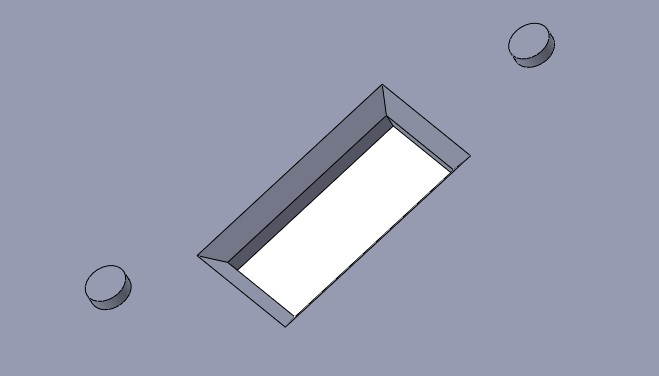
\includegraphics[width=\linewidth]{body_ppg}
			\caption{نمای درونی}
			%\label{fig:oled_image}
		\end{subfigure} 
		\begin{subfigure}{0.45\textwidth}
			\centering
			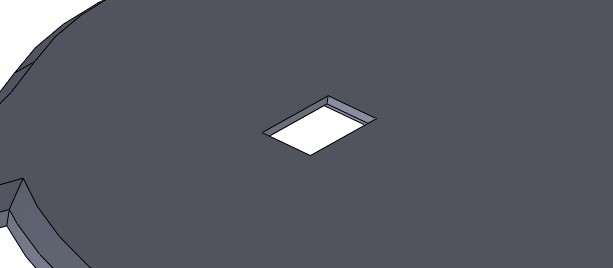
\includegraphics[width=\linewidth]{body_ppg2}
			\caption{نمای بیرونی}
			%\label{fig:oled_real}
		\end{subfigure}
		\caption{تصاویر محل نصب حسگر \lr{PPG}}
		\label{fig:body-ppg}
	\end{figure}

\end{enumerate}

در نهایت تصویر دریچه‌ی پشتی در شکل \ref{fig:body-back-reel} دیده می‌شود. چاپ این نسخه نیز توسط شرکت \lr{PCBWay}\cite{PCBWay} به رایگان انجام شده است. جنس بدنه از رزین است که باعث می‌شود شفاف باشد و داخل آن دیده شود.

	\begin{figure}[h]
		\centering
		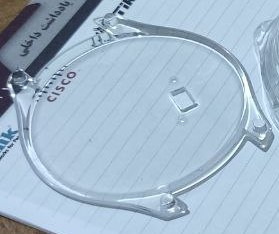
\includegraphics[width=0.5\linewidth]{body_real4}
		\caption{تصویر چاپ شده‌ی نسخه‌ی نهایی دریچه‌ی پشتی از جنس رزین و شفاف}
		\label{fig:body-back-reel}
	\end{figure}

\section{اتصالات}
 تمامی اتصالات مکانیکی در این بخش توضیح داده می‌شود.
 
 \subsection{کلیدهای لمسی}
 باید چهار قطعه سیم به شکل حلقوی سیم پیچی شده و از داخل به بدنه‌ی اصلی چسبانده شود. بدین منظور از سیم‌های وایر رپ\footnote{\lr{Wire wrap}} استفاده شده است. همانطور که در شکل \ref{fig:conn-touch} دیده می‌شود این سیم‌ها به کمک چسب نواری به بدنه‌ی اصلی متصل شده‌اند. کلیدهای لمسی به کمک خاصیت خازنی کار می‌کنند. سر دیگر سیم‌ها به محل اتصال کلیدهای لمسی در شکل \ref{fig:touch_real} لحیم می‌شوند.
 
با توجه به این که می‌توان لایه‌ی نازک فوقانی را به صورت یک دی‌الکتریک برای خازن در نظر گرفت، می‌توان گفت با اینکه کلیدها پشت صفحه نصب شده‌اند اما باز هم به درستی کار خواهند کرد. 

	\begin{figure}[h]
		\centering
		\begin{subfigure}{0.45\textwidth}
			\centering
			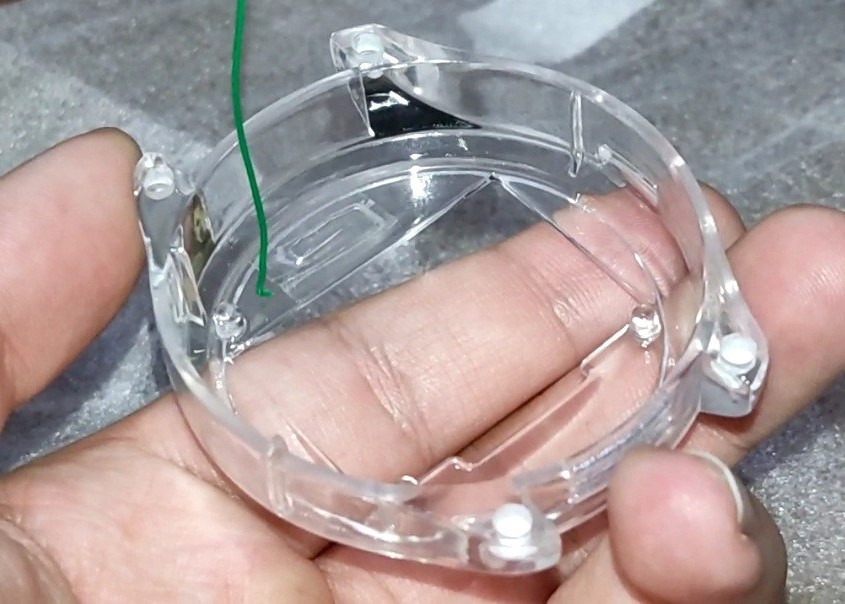
\includegraphics[width=\linewidth]{conn-touch}
			\caption{یک کلید نصب شده بر پشت سطح فوقانی}
			%\label{fig:oled_image}
		\end{subfigure} 
		\begin{subfigure}{0.45\textwidth}
			\centering
			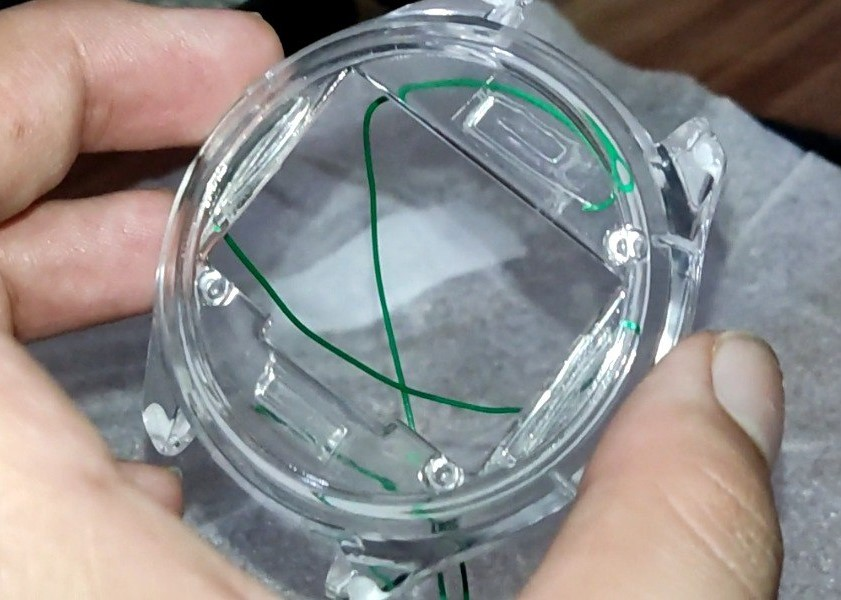
\includegraphics[width=\linewidth]{conn-touch2}
			\caption{چهار کلید نصب شده در چهار سمت بدنه}
			%\label{fig:oled_real}
		\end{subfigure}
		\caption{تصاویر اتصال کلیدهای لمسی به بدنه}
		\label{fig:conn-touch}
	\end{figure}

\subsection{صفحه نمایش}
همانطور که بالاتر بحث شد، صفحه نمایش با قرار گیری در سه استوانه‌ی موجود در بدنه سر جای خود محکم می‌شود. شکل \ref{fig:conn-oled} گویای این موضوع است.

	\begin{figure}[h]
		\centering
		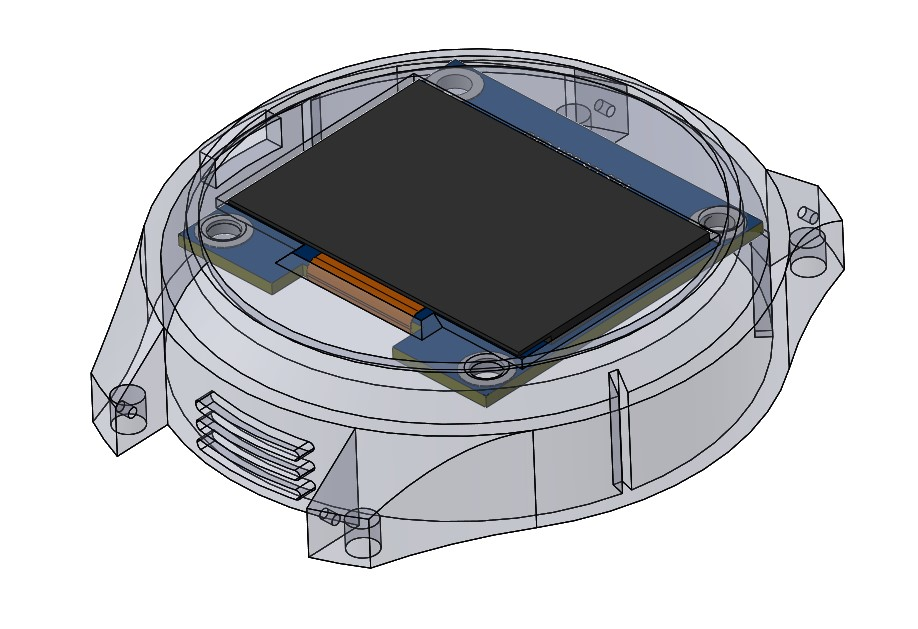
\includegraphics[width=0.5\linewidth]{conn_oled}
		\caption{تصویر اتصال صفحه نمایش به بدنه}
		\label{fig:conn-oled}
	\end{figure}

\subsection{\pcbf}
همانطور که بالاتر بحث شد، \pcbf با قرار گیری روی سه زائده‌ی موجود در بدنه سر جای خود محکم می‌شود. شکل \ref{fig:conn-pcb} گویای این موضوع است.

علت آن که برای اتصال صفحه نمایش یک استوانه از چهار استوانه حذف شده است آن است که استوانه‌ی حذف شده دقیقا بالای موتور ایجاد لرزش قرار داشت و در صورت وجود، به آن گیر می‌کرد و مانع جا گیری صحیح \pcbf می‌شد.

برای جلوگیری از اتصال ناخواسته و اتصال کوتاه بین صفحه نمایش و \pcbf، یک ورق نازک فوم بین این دو قرار گرفته است.

	\begin{figure}[h]
		\centering
		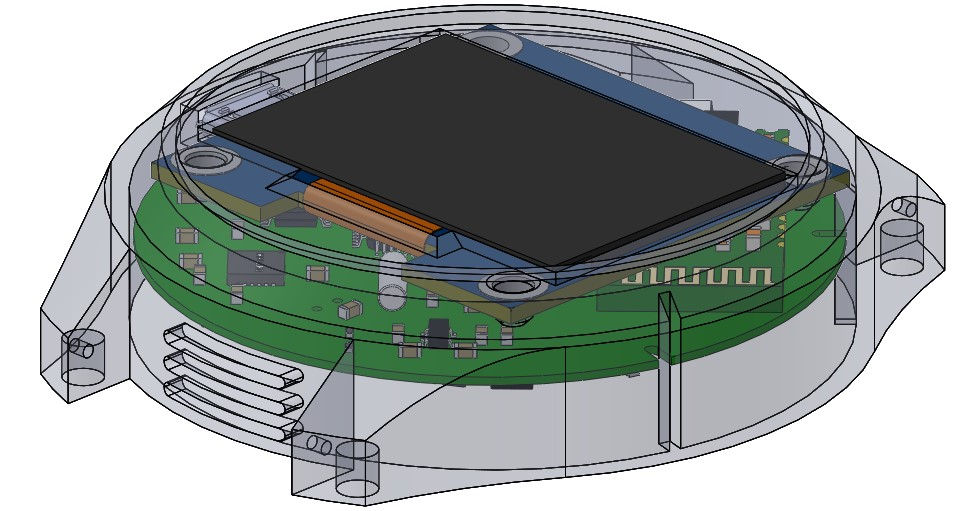
\includegraphics[width=0.5\linewidth]{conn_pcb}
		\caption{تصویر اتصال \pcbf به بدنه}
		\label{fig:conn-pcb}
	\end{figure}

\subsection{باتری}
باتری ساعت به کمک نوار چسب به \pcbf می‌چسبد و در جای خود محکم می‌شود. سیم‌های آن به محل خود لحیم شده و اتصال برقرار می‌شود. شکل \ref{fig:conn-battery} این اتصال را نشان می‌دهد.

	\begin{figure}[h]
		\centering
		\begin{subfigure}{0.5\textwidth}
			\centering
			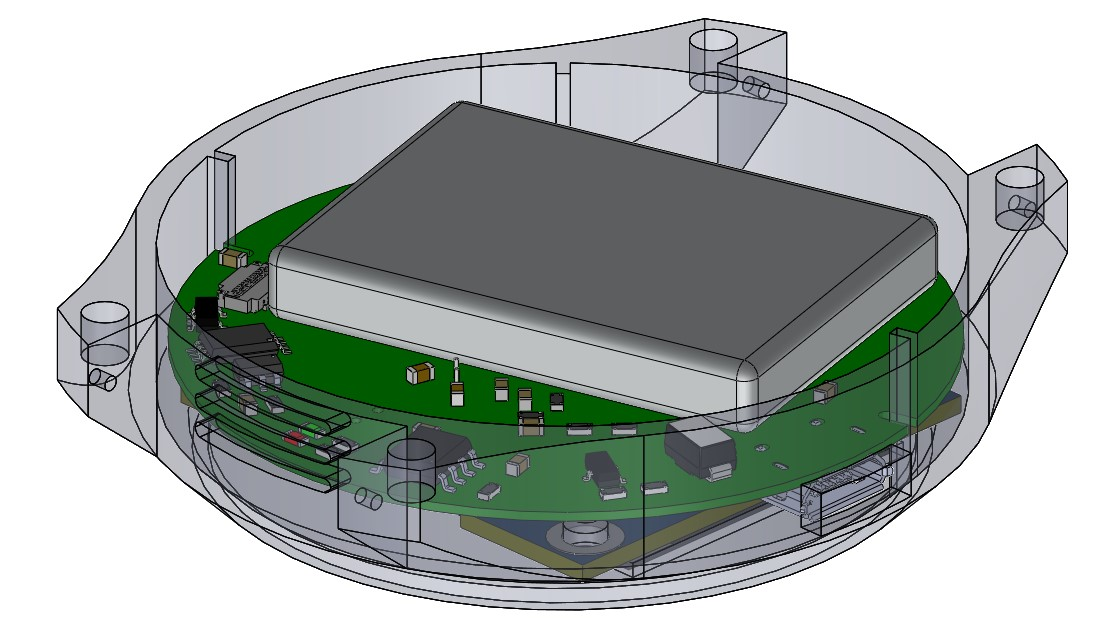
\includegraphics[width=\linewidth]{conn_battery}
			\caption{تصویر اتصال باتری در سالیدورکز}
			%\label{fig:oled_image}
		\end{subfigure} 
		\begin{subfigure}{0.4\textwidth}
			\centering
			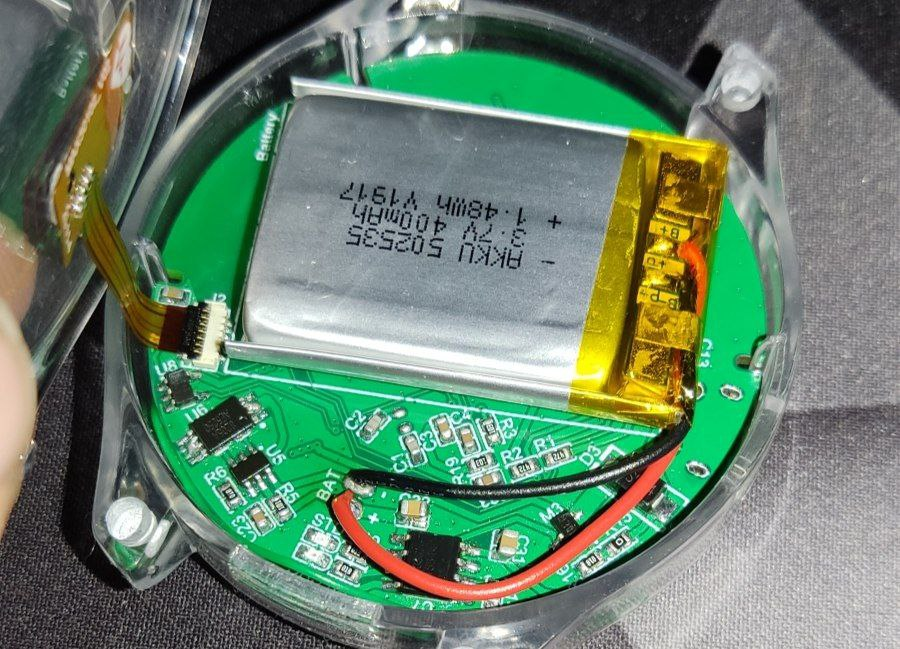
\includegraphics[width=\linewidth]{conn_battery2}
			\caption{تصویر واقعی باتری و اتصال آن}
			%\label{fig:oled_real}
		\end{subfigure}
		\caption{تصاویر اتصال باتری}
		\label{fig:conn-battery}
	\end{figure}

\subsection{حسگر \lr{PPG}}
این حسگر روی دریچه‌ی پشتی نصب می‌شود. همانطور که در شکل \ref{fig:conn-ppg} مشاهده می‌شود این حسگر به دریچه متصل است و سمت دیگر آن در جای مخصوص خود به \pcbf اتصال دارد. سوراخ مستطیل شکل روی دریچه و ضخامت مناسب آن باعث می‌شود سطح حسگر مماس سطح بیرونی دریچه باشد. اینگونه نه بیرون زدگی دارد تا آسیب ببیند و نه سطح آن از پوست فاصله می‌گیرد.

\begin{figure}[h]
	\centering
	\begin{subfigure}{0.405\textwidth}
		\centering
		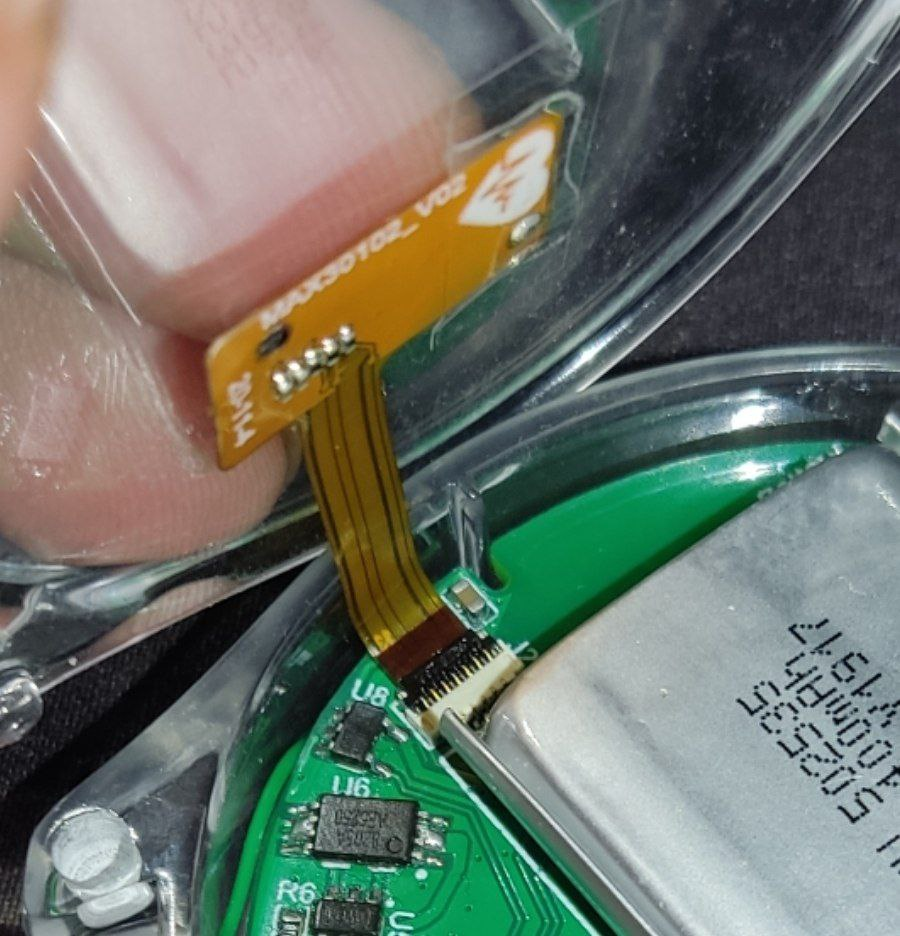
\includegraphics[width=\linewidth]{conn_ppg}
		\caption{نمای درونی}
		%\label{fig:oled_image}
	\end{subfigure} 
	\begin{subfigure}{0.4\textwidth}
		\centering
		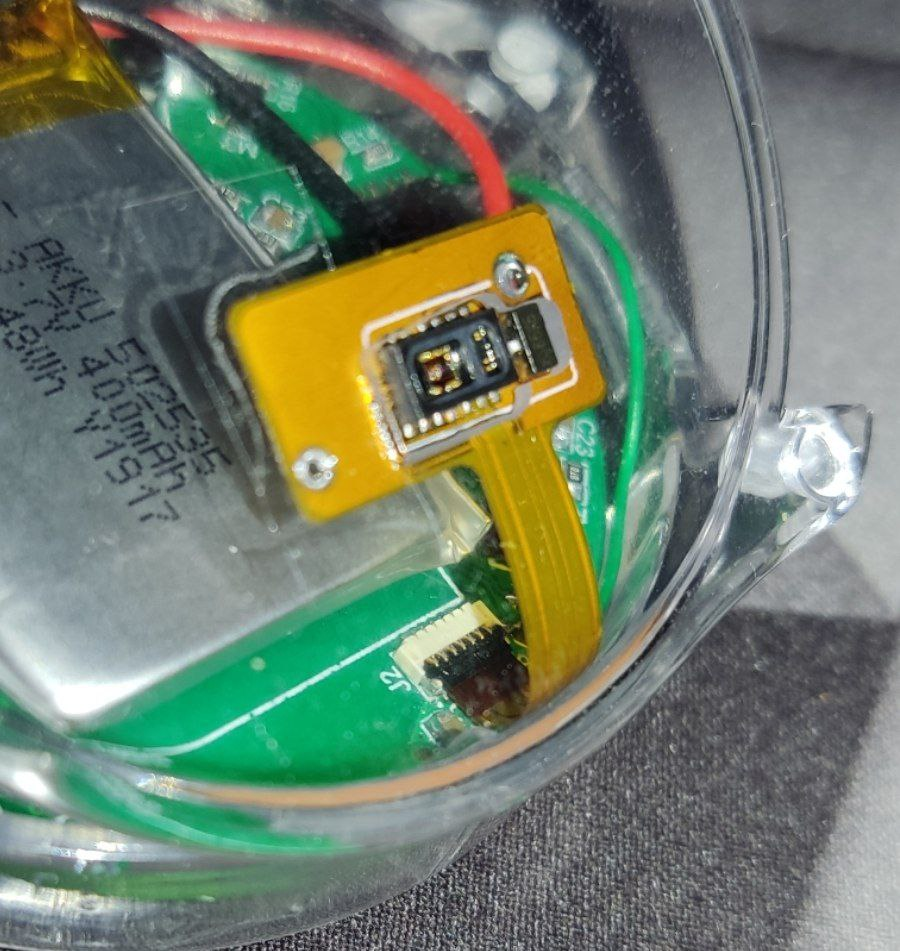
\includegraphics[width=\linewidth]{conn_ppg2}
		\caption{نمای بیرونی}
		%\label{fig:oled_real}
	\end{subfigure}
	\caption{تصاویر اتصال حسگر \lr{PPG}}
	\label{fig:conn-ppg}
\end{figure}

\subsection{دریچه‌ی پشتی}
دریچه‌ی پشتی مطابق با شکل \ref{fig:conn-back} به کمک چهار استوانه‌ی موجود روی آن به بدنه‌ی اصلی متصل می‌شود.

	\begin{figure}[h]
		\centering
		\begin{subfigure}{0.5\textwidth}
			\centering
			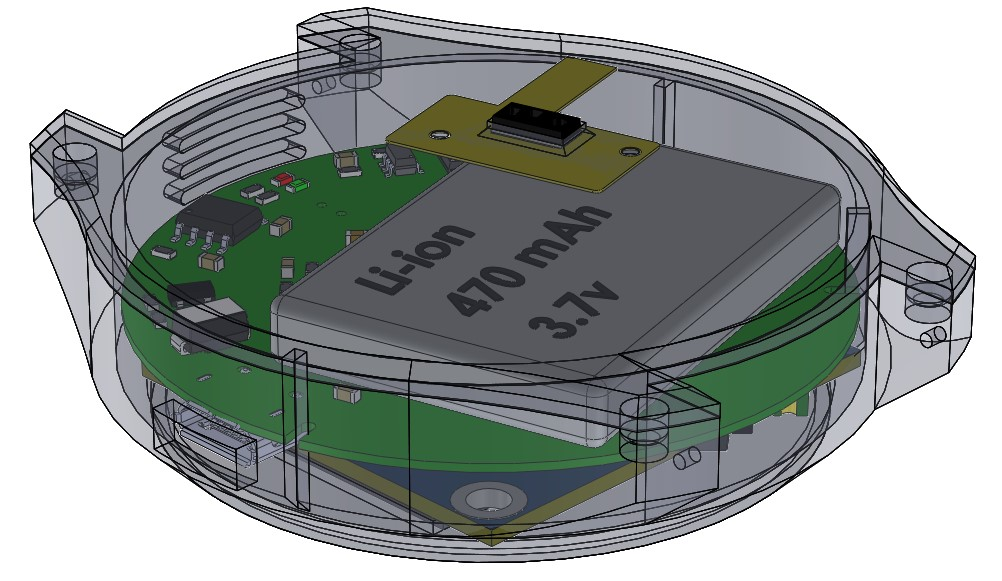
\includegraphics[width=\linewidth]{conn_back}
			\caption{تصویر اتصال دریچه در سالیدورکز}
			%\label{fig:oled_image}
		\end{subfigure} 
		\begin{subfigure}{0.4\textwidth}
			\centering
			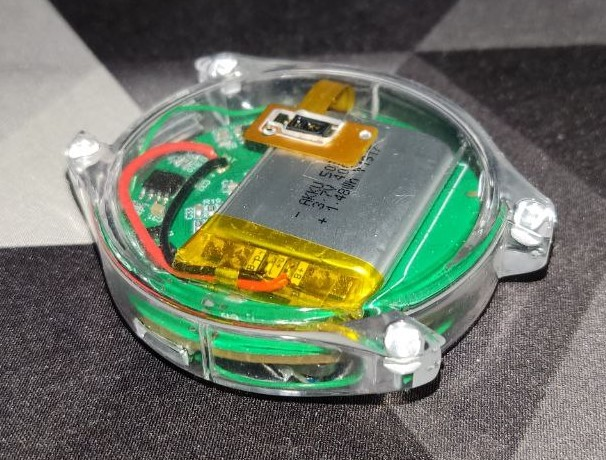
\includegraphics[width=\linewidth]{conn_back2}
			\caption{تصویر واقعی دریچه و اتصال آن}
			%\label{fig:oled_real}
		\end{subfigure}
		\caption{تصاویر اتصال دریچه‌ی پشتی}
		\label{fig:conn-back}
	\end{figure}

در نهایت بدنه و مکانیک ساعت تکمیل شد و ظاهر نهایی ساعت به شکل \ref{fig:body-final} در آمد.

	\begin{figure}[h]
		\centering
		\begin{subfigure}{0.4\textwidth}
			\centering
			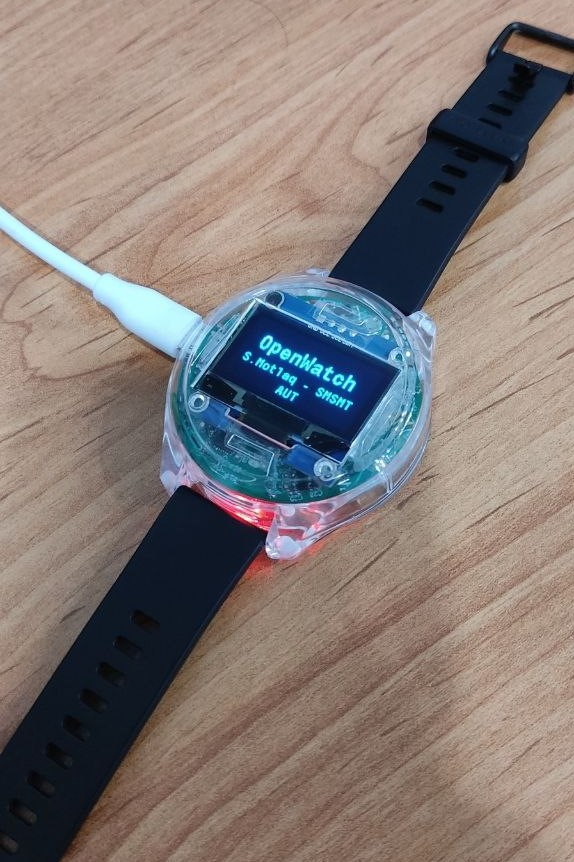
\includegraphics[width=\linewidth]{body_full}
			\caption{نمای رو}
			%\label{fig:oled_image}
		\end{subfigure} 
		\begin{subfigure}{0.4\textwidth}
			\centering
			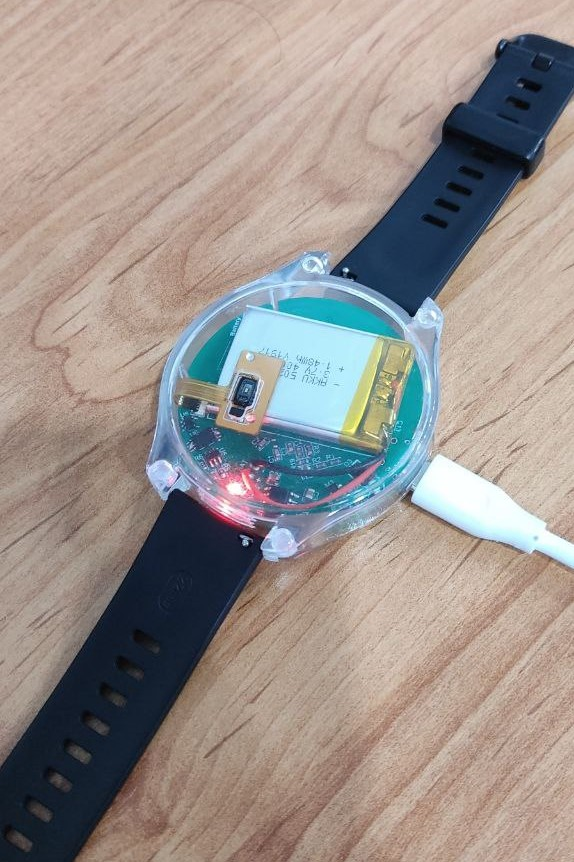
\includegraphics[width=\linewidth]{body_full2}
			\caption{نمای زیر}
			%\label{fig:oled_real}
		\end{subfigure}
		\caption{تصاویر بدنه‌ی کامل}
		\label{fig:body-final}
	\end{figure}